\documentclass[10pt,twocolumn]{article}
% ---------- Page and type ----------
\usepackage[letterpaper, left=0.7in, right=0.7in, top=0.85in, bottom=0.85in, headsep=0.2in, footskip=0.35in, columnsep=0.25in]{geometry}
\usepackage{amsmath,amssymb}
\usepackage{unicode-math}
\setmainfont{LibertinusSerif}[Extension=.otf, UprightFont=*-Regular, BoldFont=*-Semibold, ItalicFont=*-Italic, BoldItalicFont=*-SemiboldItalic]
\setsansfont{LibertinusSans}[Extension=.otf, UprightFont=*-Regular, BoldFont=*-Bold, ItalicFont=*-Italic]
\setmonofont{LibertinusMono-Regular.otf}[Scale=0.88]
\setmathfont{LibertinusMath-Regular.otf}
\usepackage[final]{microtype}
\usepackage[table]{xcolor}
\definecolor{ink}{HTML}{1F1F1F}
\definecolor{accent}{HTML}{0F7EA3}
\definecolor{crimson}{HTML}{C2185B}
\definecolor{violet}{HTML}{6250D6}
\definecolor{muted}{HTML}{6B6B68}
\definecolor{paper2}{HTML}{F3F7F9}
\definecolor{paper3}{HTML}{F5F4F1}
\definecolor{rule}{HTML}{BDBDB8}
\definecolor{surface}{HTML}{EFECE7}
\definecolor{surfaceline}{HTML}{B8B1A6}
\definecolor{earth}{HTML}{5F9EC4}
\definecolor{land}{HTML}{86B394}

% ---------- Figures, tables, units ----------
\usepackage{graphicx}
\usepackage{booktabs,tabularx,multirow,array,makecell}
\usepackage{siunitx}
\sisetup{group-separator={,}, group-minimum-digits=4, per-mode=symbol, detect-all, range-phrase={--}, range-units=single}
\usepackage{tikz}
\usetikzlibrary{positioning,arrows.meta,fit,backgrounds,calc,shapes.geometric}
\usepackage{pgfplots}
\pgfplotsset{compat=1.18}
\usepackage[font=footnotesize, labelfont={bf,sf}, labelsep=period, skip=4pt]{caption}
\usepackage{subcaption}
\usepackage{float}
\usepackage{placeins}
\setcounter{dbltopnumber}{2}
\renewcommand{\dbltopfraction}{0.92}
\renewcommand{\dblfloatpagefraction}{0.8}
\renewcommand{\topfraction}{0.9}
\renewcommand{\bottomfraction}{0.6}
\renewcommand{\textfraction}{0.08}
\renewcommand{\floatpagefraction}{0.75}
\setcounter{topnumber}{3}
\setcounter{totalnumber}{4}
\setlength{\floatsep}{9pt plus 2pt minus 2pt}
\setlength{\textfloatsep}{11pt plus 2pt minus 3pt}
\setlength{\intextsep}{9pt plus 2pt minus 2pt}
\usepackage{algorithm}
\usepackage[noend]{algpseudocode}
\usepackage{enumitem}
\setlist{itemsep=1pt, topsep=3pt, parsep=1pt, leftmargin=1.4em}
\usepackage{xspace}

% ---------- Headings ----------
\usepackage[explicit]{titlesec}
\titleformat{\section}{\normalfont\fontsize{11}{13}\selectfont\bfseries\color{ink}}{\thesection}{0.6em}{#1}
\titleformat{\subsection}{\normalfont\normalsize\bfseries\color{ink}}{\thesubsection}{0.6em}{#1}
\titleformat{\subsubsection}[runin]{\normalfont\normalsize\itshape}{}{0pt}{#1.}
\titlespacing*{\section}{0pt}{1.6ex plus .4ex minus .2ex}{0.8ex plus .2ex}
\titlespacing*{\subsection}{0pt}{1.3ex plus .3ex minus .2ex}{0.5ex plus .1ex}
\titlespacing*{\subsubsection}{0pt}{1ex plus .3ex minus .2ex}{0.6em}
\titleformat{\paragraph}[runin]{\normalfont\normalsize\bfseries}{}{0pt}{#1}
\titlespacing*{\paragraph}{0pt}{0.9ex plus .3ex minus .2ex}{0.6em}
\usepackage{fancyhdr}
\pagestyle{fancy}
\fancyhf{}
\renewcommand{\headrulewidth}{0pt}
\fancyhead[L]{\footnotesize\sffamily\color{muted}Marswalk: Earth-independent planning and guidance for walking EVAs on Mars}
\fancyhead[R]{\footnotesize\sffamily\color{muted}\thepage}
\fancypagestyle{plain}{\fancyhf{}\fancyfoot[C]{\footnotesize\sffamily\color{muted}\thepage}}

% ---------- References and links ----------
\usepackage[numbers, sort&compress]{natbib}
\setlength{\bibsep}{2pt plus 1pt}
\renewcommand{\bibfont}{\footnotesize}
\usepackage[hyphens]{url}
\def\UrlBreaks{\do\/\do\-\do\_}
\Urlmuskip=0mu plus 1mu
\usepackage[colorlinks=true, linkcolor=accent, citecolor=accent, urlcolor=accent, pdfusetitle, bookmarksnumbered]{hyperref}
\usepackage[nameinlink, capitalise, noabbrev]{cleveref}
\crefname{algorithm}{Algorithm}{Algorithms}
\urlstyle{same}

% ---------- Macros ----------
\newcommand{\Marswalk}{Marswalk\xspace}
\DeclareRobustCommand{\stayin}{\textsc{stay\nobreakspace in}\xspace}
\DeclareRobustCommand{\go}{\textsc{go}\xspace}
\DeclareRobustCommand{\nogo}{\textsc{no\nobreakdash-go}\xspace}
\DeclareRobustCommand{\autonomous}{\textsc{autonomous}\xspace}
\newcommand{\code}[1]{\texttt{#1}}
\newcommand{\gmars}{g_{\mathrm{M}}}
\newcolumntype{L}{>{\raggedright\arraybackslash}X}
\newcolumntype{C}{>{\centering\arraybackslash}X}
\renewcommand{\arraystretch}{1.12}
\setlength{\parskip}{0pt}
\frenchspacing
\setlength{\emergencystretch}{1.5em}
\widowpenalty=10000
\clubpenalty=10000

\graphicspath{{../figs/}}

% ---------- Authors: edit this block to finalise the author list ----------
\newcommand{\PaperAuthors}{%
  \begin{tabular}{@{}c@{\hspace{2.2em}}c@{\hspace{2.2em}}c@{}}
    Kumar Sashank Ghanta & Ivan & Mirim \\[-1pt]
    {\footnotesize\color{muted}\href{mailto:kumarsashank2003@gmail.com}{kumarsashank2003@gmail.com}} &
    {\footnotesize\color{muted}\href{mailto:ivanchen858@gmail.com}{ivanchen858@gmail.com}} &
    {\footnotesize\color{muted}\href{mailto:firepunch119@gmail.com}{firepunch119@gmail.com}} \\[5pt]
  \end{tabular}\\
  \begin{tabular}{@{}c@{\hspace{2.2em}}c@{}}
    Michelle & George \\[-1pt]
    {\footnotesize\color{muted}\href{mailto:michelle.wang.cs@gmail.com}{michelle.wang.cs@gmail.com}} &
    {\footnotesize\color{muted}\href{mailto:georgepostica7@gmail.com}{georgepostica7@gmail.com}} \\
  \end{tabular}}
\newcommand{\PaperAffiliation}{Team NASASpaceHacks \textperiodcentered{} NASA International Space Apps Challenge 2026 \textperiodcentered{} Toronto, Canada}
\newcommand{\PaperRepo}{\url{https://github.com/NASASpaceHacks/NASASpaceHacks2026}}

\hypersetup{pdftitle={Marswalk: Earth-Independent Planning and Guidance for Walking EVAs on Mars}, pdfauthor={Kumar Sashank Ghanta, Ivan, Mirim, Michelle, George}, pdfkeywords={Mars, extravehicular activity, EVA planning, traverse planning, route planning, orienteering, metabolic cost, space suit, autonomy, HiRISE, Curiosity, Gale crater}}

\begin{document}
\thispagestyle{plain}

\twocolumn[{%
\begin{center}
  {\sffamily\small\color{muted} Research paper \textperiodcentered{} NASA Space Apps Challenge 2026: Interplanetary Survival Guide, Martian Map\par}
  \vspace{10pt}
  {\LARGE\bfseries\color{ink} Marswalk: Earth-Independent Planning and\\[3pt] Guidance for Walking EVAs on Mars\par}
  \vspace{12pt}
  {\large \PaperAuthors\par}
  \vspace{4pt}
  {\small\color{muted} \PaperAffiliation\par}
  \vspace{2pt}
  {\small \PaperRepo\par}
  \vspace{2pt}
  {\small\color{muted} 15 November 2026\par}
\end{center}

\vspace{6pt}
\noindent\begin{minipage}{\textwidth}
\setlength{\parindent}{0pt}
\begin{center}\begin{minipage}{0.92\textwidth}
\small
\textbf{Abstract.} Astronauts on Mars will have to plan and carry out their own walks outside, because Earth cannot help in real time. Two gaps stand in the way. First, extravehicular activities (EVAs) are routed from Earth today. From Mars, asking a question and hearing back takes up to 44 minutes, contact is lost for weeks around solar conjunction, and an onboard solar-storm alarm leaves only about 30 minutes to reach shelter, so Earth is too slow for an emergency. Second, the route planners that already run on Mars are built for rovers. They model wheels and slopes, not a suited human's oxygen time, suit heat or walk back to shelter. We present \Marswalk, which plans human routes on Mars itself, in milliseconds, with no Earth in the loop. In the habitat, it plans walks on a terrain model fused from NASA and ESA orbital and rover data and checks every plan against twelve sourced EVA constraints, including suit heat, walk-back time, time to shelter and radio contact. A separate simulator re-checks each plan, and the engine explains its verdict. A signed route of about 11\,kB goes to the astronaut's phone AR navigator, which estimates position without GPS (in simulation today), re-routes locally and keeps guiding when the link drops. A suit hardware concept adds boot-mounted inertial sensors, camera-to-orbital-map matching and a helmet waveguide display. At Gale crater, a slope-only planner broke at least one constraint in 199 of 200 simulated walks. \Marswalk re-plans mid-walk in a median of 8.3\,ms on a laptop, and its walking model has a 10.6\% mean error against NASA suited-walking data at 0.22--0.32\,$g$. An independently written checker agreed with its verdicts on 23 of 24 walks, and staging from a pressurized rover turned an infeasible habitat walk into a six-stop plan. \Marswalk is a research prototype tested in simulation.

\vspace{5pt}
\textbf{Keywords:} Mars; extravehicular activity; traverse planning; crew autonomy; suit thermal limits; GPS-free navigation; augmented reality; Gale crater.
\end{minipage}\end{center}
\end{minipage}
\vspace{4pt}
\vspace{10pt}
}]

\section{Introduction}
\label{sec:intro}

On the Moon, an astronaut is a radio call away from flight controllers who watch every consumable and every step. On Mars that loop breaks. One-way light time to Earth ranges from about 3 to 22 minutes, and around each solar conjunction, every 26 months, when the Sun passes between Earth and Mars, it blocks contact for roughly two to three weeks \citep{mcbrayer2022comms}. NASA's exploration EVA concept of operations (ConOps) expects Mars crews to ``be more involved in planning their EVAs than as is currently done on ISS,'' using ``crew input, ground based planners, and automated planning tools'' under a delay of ``\textasciitilde4 and 20 minutes'' \citep{coan2020conops}. A recent review of planetary EVA tools finds that operational work has focused ``almost exclusively on microgravity rather than planetary surface operations'' \citep{elston2026review}.

Two gaps stand between today's tools and that need.
\emph{Gap~1: walks are routed from Earth.} EVA planning and monitoring are ground-based; NASA's EVA Mission System Software describes its role as ``empowering ground-based flight controllers'' \citep{miller2026emss}. From Mars, a question and its answer take up to 44 minutes. An onboard solar-particle alarm leaves only about 30 minutes to reach shelter \citep{lowe2025nowcast}. Earth therefore cannot re-route a walk in an emergency.
\emph{Gap~2: the planners on Mars are built for rovers.} The route planners that already run on Mars drive rovers \citep{carsten2009,toupet2026enav}. They model wheels, slip and slope, not a suited human's oxygen time, metabolic heat or walk back to shelter. Map portals show the data but plan nothing \citep{marstrek,mmgis}. Energy-optimal walking planners model effort, but not the full set of EVA constraints or guidance on Mars \citep{johnson2010sextant,penaasensio2024moonpath}.
Closing both gaps requires a crew-side tool that is
\textbf{R1}~\emph{Earth-independent}, planning and guiding on Mars without internet access;
\textbf{R2}~\emph{constraint-checked} against documented EVA limits, with ``do not go out'' always an acceptable answer;
\textbf{R3}~\emph{physiological}, following suited metabolism and suit heat rejection at Mars gravity;
\textbf{R4}~\emph{explainable} to a non-expert; and
\textbf{R5}~\emph{executable under link loss}, verified on arrival and still guiding the astronaut home without a link or GPS.

We present \Marswalk, built for the 2026 NASA International Space Apps Challenge (``Interplanetary Survival Guide: Martian Map''). In \Marswalk, the intravehicular (IV) crewmember in the habitat plans a walk on a 5\,km\,$\times$\,5\,km terrain model of Gale crater. The model fuses NASA and ESA orbital and rover data and includes Curiosity's 2025--26 boxwork campaign. The engine selects science stations, routes between them and checks the plan against twelve sourced constraints. A separate simulator then re-checks every plan before it is returned, and the engine explains the verdict. The confirmed plan is signed and sent as a package of about 11\,kB to the astronaut's phone-based augmented-reality (AR) navigator. The navigator estimates position without GPS, today from simulated drift and fixes, and keeps guiding when the link drops (\cref{fig:arch}). Our contributions are:
\begin{enumerate}[label=(\arabic*)]
  \item A formulation of crew-side Mars EVA planning as constrained orienteering on real terrain. Every constraint carries a source and an evidence class, and \stayin is a first-class result (\cref{sec:system}).
  \item A route engine that couples a suited metabolic model at Mars gravity with a suit heat-rejection governor. It computes one-to-many safety fields, selects stations with a labelled dynamic program that is exact over precomputed legs, re-checks plans in a separate time-stepped simulator, and explains verdicts counterfactually (\cref{sec:engine}).
  \item An Earth-independent execution path: a signed, compact route package with a conservative coarse safety grid, and a navigator with constant-time safety lookups that becomes autonomous on link loss. It is completed by a GPS-free positioning design and a suit hardware concept (\cref{sec:system,sec:interfaces,sec:hardware}).
  \item An evaluation built from public data. We compare the models with measured NASA data, quantify planning impact and parameter sensitivity over 460 simulated EVAs, cross-check verdicts against an independently written checker, and time the end-to-end system (\cref{sec:eval}).
\end{enumerate}
\Marswalk is a research prototype tested in simulation, not with suited people, real radios or EVA operators, and nothing in it is operational guidance. Its code, site-pack manifests and check scripts are open source.

\section{Related work}
\label{sec:related}

\paragraph{EVA planning and operations.} Apollo traverses were planned on Earth well in advance and bounded by how far the crew could walk back to the lunar module if the rover failed \citep{benjamin1969apollo,norcross2009ewt}. Analog campaigns built the ground side of exploration EVA: traverse tools in NASA's Exploration Ground Data Systems \citep{lee2013xgds}, science operations under latency in BASALT \citep{lim2019basalt,beaton2019}, and lunar EVA planning in the Joint EVA Test Team campaigns \citep{caswell2023jett3}. NASA's EVA Mission System Software estimates timelines and science coverage for Artemis; its developers describe it as ``empowering ground-based flight controllers'' \citep{miller2026emss}. Flight-operations work lists the constraints a surface traverse must respect \citep{caswell2025eva}, and the Artemis~III tenets bound walking EVAs to 2\,km from the lander \citep{kagey2023tenets}.

\paragraph{Traverse planners for suited humans.} SEXTANT computes minimum-distance, minimum-time and minimum-energy traverses for suited astronauts and reports walk-back from any point \citep{johnson2010sextant,norheim2018sextant}. \Citet{penaasensio2024moonpath} find minimum-metabolic-workload paths at the lunar south pole, and \citet{broddrick2024} cast science-yield optimization as a mixed-integer linear program. These planners build on load-carriage metabolic models \citep{pandolf1977,santee2001} that NASA has adapted for suited traverse planning \citep{kim2024metabolic}, and on suited and partial-gravity locomotion data \citep{norcross2010level,norcross2010incline,carr2007framework,kluis2025}.

\paragraph{Rover navigation and orienteering.} Planetary rovers plan on terrain cost maps, from Field D$^\ast$ on the Mars Exploration Rovers \citep{ferguson2006,carsten2009} and D$^\ast$ Lite re-planning \citep{koenig2002dstar} to Perseverance's enhanced autonomous navigation \citep{toupet2026enav} and learned heuristics \citep{daftry2022}. These planners have no metabolic budget and no walk home. Choosing stops within a time budget is the orienteering problem \citep{golden1987,vansteenwegen2011,gunawan2016}. Its exact dynamic program over subsets goes back to Bellman and to Held and Karp \citep{bellman1962,heldkarp1962}, and Pareto labels come from resource-constrained shortest paths \citep{feillet2004,irnich2005}. Explaining plans is the subject of explainable planning \citep{chakraborti2020}.

\paragraph{Mars data, radiation and displays.} Mars Trek and MMGIS serve orbital and mission data \citep{marstrek,mmgis}. Curiosity's Radiation Assessment Detector (RAD) has measured the surface dose \citep{hassler2014}, its dependence on pressure and solar modulation \citep{guo2015}, and its reduction by nearby terrain \citep{guo2026}. \Citet{lowe2025nowcast} propose nowcasting solar energetic particle (SEP) events from the onboard dose rate. NASA's Joint Augmented Reality work is developing suit navigation displays and notes that ``a seamless suit-integrated AR solution does not yet exist'' \citep{miller2022ar}.

\Cref{tab:related} summarizes our reading. \Marswalk's novelty lies in combining these elements into one offline system and in the checking and hand-off steps between them, not in any single algorithm.

\DeclareRobustCommand{\capfull}{\tikz[baseline=-0.6ex]\fill[ink] (0,0) circle (2.3pt);}
\DeclareRobustCommand{\cappart}{\tikz[baseline=-0.6ex]{\draw[ink, line width=0.55pt] (0,0) circle (2.3pt); \fill[ink] (0,0) -- (90:2.3pt) arc (90:270:2.3pt) -- cycle;}}
\DeclareRobustCommand{\capnone}{\tikz[baseline=-0.6ex]\draw[ink, line width=0.5pt] (0,0) circle (2.3pt);}
\begin{table*}[t]
  \centering\footnotesize\renewcommand{\arraystretch}{1.05}
  \caption{Capabilities against requirements R1--R5, in our reading of public sources (judgments, not measurements). \capfull\ documented; \cappart\ partly; \capnone\ not found in public sources, which does not mean absent. \Marswalk's explanations have not been evaluated with users, and its link-loss behaviour has been tested only over a simulated link.}
  \label{tab:related}
  \begin{tabular}{@{}l c c c c c c@{}}
    \toprule
    & R1 & R2 & \multicolumn{2}{c}{R3} & R4 & R5 \\
    \cmidrule(lr){4-5}
    Tool & Earth-independent & Hard constraints & Energy & Suit heat & Explains & Link-loss execution \\
    \midrule
    Mars Trek, MMGIS \citep{marstrek,mmgis} & \capnone & \capnone & \capnone & \capnone & \capnone & \capnone \\
    EMSS traverse planning \citep{miller2026emss} & \capnone & \cappart & \capnone & \capnone & \capnone & \capnone \\
    SEXTANT \citep{johnson2010sextant,norheim2018sextant} & \capnone & \cappart & \capfull & \cappart & \capnone & \capnone \\
    Lunar metabolic paths \citep{penaasensio2024moonpath} & \capnone & \cappart & \capfull & \capnone & \capnone & \capnone \\
    Science-yield MILP \citep{broddrick2024} & \capnone & \cappart & \capnone & \capnone & \capnone & \capnone \\
    Rover planners \citep{carsten2009,toupet2026enav} & \capfull & \capfull & \capnone & \capnone & \capnone & \capfull \\
    Joint AR displays \citep{miller2022ar} & \cappart & \capnone & \capnone & \capnone & \capnone & \cappart \\
    \Marswalk & \capfull & \capfull & \capfull & \capfull & \cappart & \cappart \\
    \bottomrule
  \end{tabular}
\end{table*}

\section{System and problem}
\label{sec:system}

\begin{figure*}[t]
  \centering
  % Illustrated system architecture: asynchronous with Earth, heavy in the habitat, light on the helmet.
\begin{tikzpicture}[x=1mm, y=1mm, font=\rmfamily\scriptsize,
  callout/.style={draw=ink!55, line width=0.45pt, rounded corners=1.5pt, fill=white, align=left, inner sep=3pt,
                  execute at begin node={\hyphenpenalty=10000}},
  tag/.style={font=\rmfamily\itshape\footnotesize, text=muted},
  line/.style={draw=ink!70, line width=0.5pt},
]
% ---------------- ground and panels ----------------
\fill[paper3, rounded corners=3pt] (0,10) rectangle (37,78);
\fill[surface] (41,10) -- (41,21) .. controls (60,22.5) and (75,20.5) .. (95,21.3) .. controls (115,22.2) and (135,20.4) .. (165,21.6) -- (165,10) -- cycle;
\draw[surfaceline, line width=0.6pt] (41,21) .. controls (60,22.5) and (75,20.5) .. (95,21.3) .. controls (115,22.2) and (135,20.4) .. (165,21.6);
\draw[ink!30, dashed, line width=0.5pt] (39,12) -- (39,78);
\node[font=\rmfamily\bfseries\footnotesize, text=ink, anchor=north west] at (1.5,77) {Earth};
\node[font=\rmfamily\bfseries\footnotesize, text=ink, anchor=north west] at (41.5,77) {Mars surface \textnormal{\color{muted}(local radio only, no internet)}};

% ---------------- Earth ----------------
\shade[ball color=earth!80!white] (18.5,47) circle (8);
\fill[land, opacity=0.85] (14.5,50.5) .. controls (17,53) and (20.5,52) .. (21,49.5) .. controls (21.5,47) and (18,46.5) .. (16.5,47.5) .. controls (15,48.5) and (13.5,49) .. (14.5,50.5) -- cycle;
\fill[land, opacity=0.85] (19.5,43.5) .. controls (21.5,44) and (23,42.5) .. (22,41) .. controls (21,40) and (19,41.5) .. (19.5,43.5) -- cycle;
\node[callout, text width=31mm, anchor=north] at (18.5,36) {\textbf{Ground support} (optional)\\ space-weather forecasts, science backroom, plan and log archive};

% ---------------- habitat ----------------
\begin{scope}[shift={(66,21.6)}]
  \fill[white] (-10,0) rectangle (10,9);
  \draw[line, fill=white] (-10,0) -- (-10,9) arc (180:0:10 and 4.5) -- (10,0);
  \draw[line] (-10,0) -- (10,0);
  \foreach \x in {-6,-1,4} \draw[ink!60, fill=paper2] (\x,4.6) circle (1.15);
  \draw[ink!60, fill=paper2, rounded corners=0.5pt] (-2.2,0) rectangle (2.2,3);
  \draw[line, line width=0.7pt] (7,11) -- (7,22);
  \draw[line, fill=white] (5.6,22) -- (8.4,22) -- (7,24) -- cycle;
  \coordinate (habmast) at (7,23);
\end{scope}
\node[font=\rmfamily\scriptsize, text=ink, align=center] at (66,15.6) {\textbf{Hab-1}\\ \textit{\color{muted}server, console}};

% ---------------- rover ----------------
\begin{scope}[shift={(104,21.9)}]
  \draw[line, fill=white] (-11,2) -- (-11,7.5) -- (6,7.5) -- (10.5,4) -- (10.5,2) -- cycle;
  \draw[ink!60, fill=paper2] (5,6.5) -- (8.2,4.2) -- (8.2,6.5) -- cycle;
  \foreach \x in {-7,0,7} {\fill[white] (\x,1.6) circle (2.3); \draw[line] (\x,1.6) circle (2.3); \fill[ink!60] (\x,1.6) circle (0.6);}
  \draw[line, line width=0.7pt] (-6,7.5) -- (-6,17);
  \draw[line, fill=white] (-7.2,17) -- (-4.8,17) -- (-6,18.8) -- cycle;
  \coordinate (rovmast) at (-6,18);
\end{scope}
\node[font=\rmfamily\scriptsize, text=ink, align=center] at (104,15.6) {\textbf{PR-1}\\ \textit{\color{muted}mobile base, relay}};

% ---------------- astronaut with phone ----------------
\begin{scope}[shift={(141,21.4)}]
  \draw[line, fill=paper3, rounded corners=0.8pt] (-6,8.5) rectangle (-3.2,16);
  \draw[line, fill=white, rounded corners=1.6pt] (-3.6,8) rectangle (3.4,16.6);
  \draw[ink!75, line width=1.6pt, line cap=round] (-1.6,8.2) -- (-2.4,0.6);
  \draw[ink!75, line width=1.6pt, line cap=round] (1.4,8.2) -- (2.6,0.6);
  \draw[line, fill=white] (0,19.6) circle (3.3);
  \fill[accent!35] (0.9,19.6) ellipse (2.0 and 1.7);
  \draw[ink!75, line width=1.3pt, line cap=round] (2.9,14.6) -- (6.2,15.9);
  \draw[line, fill=ink!85, rounded corners=0.6pt, rotate around={-12:(7.4,16.6)}] (6.1,13.6) rectangle (8.7,19.4);
  \fill[accent!70, rotate around={-12:(7.4,16.6)}] (6.5,14.3) rectangle (8.3,18.7);
  \coordinate (crew) at (2,23.5);
\end{scope}
\node[font=\rmfamily\scriptsize, text=ink, align=center] at (141,15.6) {\textbf{EV crew}\\ \textit{\color{muted}suit, phone navigator}};

% ---------------- links ----------------
\draw[accent, line width=0.9pt, -{Stealth[length=5pt]}] ($(habmast)+(1,0.8)$) .. controls (95,60) and (122,58) .. ($(crew)+(-1.2,2)$)
  node[pos=0.5, above=1pt, font=\rmfamily\scriptsize, text=accent] {signed route package, ${\approx}$11\,kB};
\draw[ink!55, line width=0.6pt, -{Stealth[length=4pt]}] ($(crew)+(-1.8,0.4)$) .. controls (120,50) and (97,51) .. ($(habmast)+(1.4,-0.6)$)
  node[pos=0.5, below=2pt, font=\rmfamily\scriptsize, text=ink!80] {telemetry, acknowledgements, crew requests};
\draw[ink!45, line width=0.5pt, densely dotted] (rovmast) -- ($(habmast)+(0.4,-1)$);
\draw[ink!45, line width=0.5pt, densely dotted] (rovmast) -- ($(crew)+(-2.5,-1.5)$);
\node[font=\rmfamily\itshape\scriptsize, text=muted, anchor=south] at ($(rovmast)+(0,0.6)$) {relay};
\draw[ink!45, line width=0.6pt, dashed, {Stealth[length=4pt]}-{Stealth[length=4pt]}] (27.2,48.5) .. controls (40,52) and (56,50.5) .. ($(habmast)+(-1.2,0.4)$)
  node[pos=0.4, below=1.5pt, align=center, font=\rmfamily\scriptsize, text=ink!80] {delayed bundles\\ 3--22\,min};

% ---------------- callouts ----------------
\node[callout, text width=40mm, anchor=north] at (66,73) {\textbf{Habitat server and console}\\ route engine, safety fields, separate simulator; Ed25519 signing key; event log for crash recovery; the IV crewmember plans, reviews and sends};
\node[callout, text width=37mm, anchor=north] at (144,73) {\textbf{Phone AR navigator}\\ verifies the route with a 32-byte key; onboard safety core; dead reckoning and local re-route; autonomous on link loss};

% ---------------- design taglines ----------------
\node[tag] at (18.5,5) {asynchronous with Earth};
\node[tag] at (66,5) {heavy in the habitat};
\node[tag] at (141,5) {light on the helmet};
\end{tikzpicture}

  \caption{\Marswalk architecture. The habitat runs the full engine and holds the signing key. The navigator carries only the signed route package, the habitat's 32-byte public key and a small safety core, so it keeps working when the habitat is silent. The pressurized rover is a mobile EVA base and a radio relay. Earth exchanges delayed bundles that nothing safety-critical reads.}
  \label{fig:arch}
\end{figure*}

\subsection{Setting and architecture}
We follow NASA's Mars Design Reference Architecture (DRA) 5.0: a crew lives in a habitat and uses pressurized rovers as mobile bases \citep{drake2009dra5}. On a given sol, two suited extravehicular (EV) crewmembers walk from an \emph{EVA base}, either the habitat (Hab-1 in our scenario) or a parked pressurized rover (PR-1). The IV crewmember inside, whom the ConOps describes as performing ``the roles of IV, Flight Director, partial EVA Officer'' \citep{coan2020conops}, plans and confirms the walk. \Marswalk follows one rule: \emph{heavy in the habitat, light on the helmet, asynchronous with Earth} (\cref{fig:arch}).

The habitat server (Node.js) runs the engine, signs route packages, serves site-pack data and appends every event to a log. The IV uses a map-based console. Each EV crewmember carries the navigator, a phone AR application (a full-screen visor display shares the same flight logic). Navigator and server exchange six message types as binary CBOR \citep{rfc8949} over a WebSocket on the habitat network: route push, acknowledgement, telemetry, alert, crew request and a 1\,Hz heartbeat. The link counts as \emph{down} after 3\,s of silence. Messages are queued while it is down and flushed once each on recovery.

A confirmed plan becomes a \emph{route package}. The package holds the stop order, the route, latest-departure (``bingo'') times and a coarse safety grid (\cref{sec:package}). The habitat signs its canonical encoding with Ed25519 \citep{bernstein2012,rfc8032}. The navigator verifies the signature, rejects stale or tampered packages, and installs a route only after the astronaut accepts it. The signature shows that a package came from the habitat server; consoles are not authenticated, so it does not prove the IV approved it. Both ends assume they will crash, since commercial electronics on Mars are exposed to radiation. The server rebuilds route, sequence and acknowledgement state from its log on restart, and the navigator restores its checkpoint (in 263\,ms for the visor in our measurement). Earth contact is optional: delayed bundles carry forecasts, plans and logs, and neither the engine nor the navigator's safety core reads Earth data.

\subsection{Plans and constraints}
The terrain is a grid of 5\,m cells $c$ with elevation $z_c$, slope $\theta_c$ and thermal inertia $I_c$, treated as an 8-connected graph. A cell is blocked if $\theta_c>\theta_{\max}=20^\circ$, if it lies in a keep-out zone, or if its data are missing; unknown terrain is never walkable. An edge is admissible only if both ends are open, its own grade satisfies $|\Delta z|\le d_h\tan\theta_{\max}$ (where $d_h$ is the horizontal step length), and, for a diagonal step, both orthogonal neighbours are open. The step rule matters because slope computed on a smoothed $3\times3$ window can hide a steep step between two cells that each pass. A plan $\mathcal{P}=(b,t_0,\sigma,\pi)$ is an EVA base $b$, a start time, an ordered sequence $\sigma$ of distinct stations (each with value $v_i$ and dwell $\delta_i$), and a path $\pi$ from $b$ through the stations and back. Walking $\pi$ at the planning pace, with rests from the heat model (\cref{sec:heat}) and dwells at stations, yields a time-stamped trajectory $\xi(\mathcal{P})$.

\Cref{tab:rules} lists the twelve constraints. Most come from public NASA EVA documents \citep{coan2020conops,kagey2023tenets,caswell2025eva,ogilvie2026marsmass,bussey2016landing}; the shelter limit comes from an analysis of Curiosity radiation data \citep{lowe2025nowcast}. Because Mars EVA flight rules are not public, we do not call these constraints flight rules. Each carries an evidence class: \textbf{M} measured, \textbf{A} analog or flight experience, \textbf{D} NASA requirement or derived from NASA documents, \textbf{E} team assumption. Eleven are hard and ten are enforced by the engine. Eight are re-checked along the trajectory by the simulator; egress and ingress set the timeline; and the keep-out is a blocked polygon. The oxygen reserve lies outside the 360-minute EVA by definition, so a plan that respects EVA duration never draws on it. Walk-back is checked at every sample as $(t-t_s)+W_b(c(t))\le A$, where $t_s$ is the start of surface time after egress, $A=300$\,min is the surface time available, and $W_b(c)$ is the time to walk from $c$ back to the base at half pace.

\begin{table*}[t]
  \centering\small
  \caption{Constraints. Check: \emph{sim} = re-checked at every step by the simulator; \emph{mask} = blocks cells or edges in every search; \emph{timeline} = sets the time budget; \emph{none} = shown but not enforced. Evidence classes are those assigned in the software. $\dagger$ team design parameter; $\ddagger$ NASA value, averaging window our assumption.}
  \label{tab:rules}
  \begin{tabularx}{\textwidth}{@{}l l c l L@{}}
    \toprule
    Constraint & Limit & Ev. & Check & Source \\
    \midrule
    Maximum slope & $20^\circ$ (cell and step) & A & mask, sim & ConOps: suited crew on slopes up to $20^\circ$ \citep{coan2020conops} \\
    Metabolic-data limit & $16.7^\circ$ & M & none & Edge of NASA suited data (30\% grade) \citep{norcross2010incline} \\
    EVA duration & 360\,min & D & sim & ConOps: $6\pm2$\,h \citep{coan2020conops} \\
    Egress and ingress & 60\,min & D & timeline & ConOps \citep{coan2020conops} \\
    Contingency O$_2$ & 60\,min & D & none & Outside the 360-min EVA; never planned into \citep{coan2020conops} \\
    Walk-back pace & $0.5\times$ nominal$^\dagger$ & E & sim & Degraded-crew return, after the Apollo walk-back limit \citep{benjamin1969apollo} \\
    Time to shelter & 30\,min & D & mask, sim & RAD-data analysis (preprint): ${\ge}30$\,min to avoid peak SEP dose \citep{lowe2025nowcast} \\
    Time out of radio contact & 10\,min$^\dagger$ & E & sim & Flight-operations constraint, max time without line of sight \citep{caswell2025eva} \\
    Daylight & sun $\ge5^\circ$$^\dagger$ & E & sim & No nominal night EVAs \citep{drake2009dra5add} \\
    Suit heat rejection & 352\,W (30-min avg.) & D$^\ddagger$ & sim & Sizing average for future suits, 1,200\,BTU/h \citep{ogilvie2026marsmass} \\
    Distance from base & 2,000\,m & D & mask, sim & Artemis~III tenets: walking EVAs within 2\,km \citep{kagey2023tenets} \\
    Landing-plume keep-out & 1,000\,m & D & mask & ``1000\,m radius plume ejecta hazard zone'' \citep{bussey2016landing} \\
    \bottomrule
  \end{tabularx}
\end{table*}

Among plans whose trajectories satisfy every hard constraint, \Marswalk maximizes total science value $\sum_{i\in\sigma}v_i$ and breaks ties by earlier return. If no plan is feasible the answer is \stayin, which satisfies every trajectory constraint trivially. This is an orienteering problem with state-dependent travel times, because rests depend on the suit's heat history, and with constraints evaluated along the whole trajectory. Beyond the plan, R4 and R5 require a binding constraint, a reason for every dropped station, bingo times, margins over time and a compact verifiable package.

\section{A multi-mission site pack}
\label{sec:data}

\begin{figure*}[t]
  \centering
  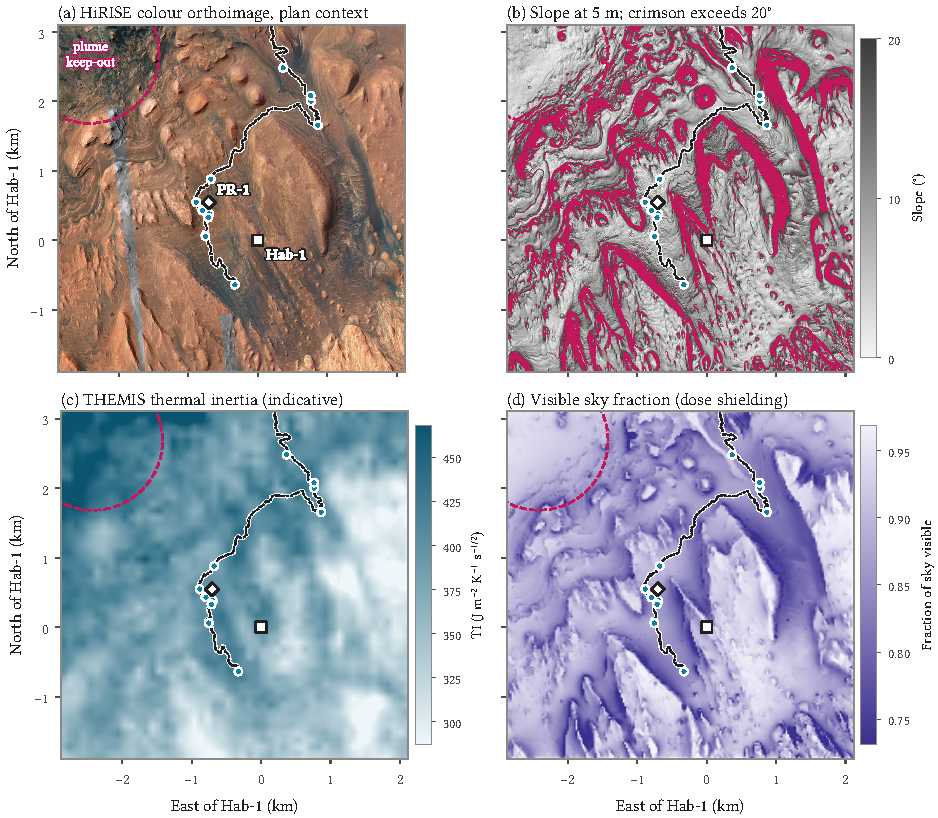
\includegraphics[width=0.6\textwidth]{site.pdf}
  \caption{The Gale study area (5\,km\,$\times$\,5\,km) in the \code{gale-v1} site pack, in kilometres relative to the scenario habitat. Dotted line: Curiosity's traverse; cyan dots: the twelve candidate stations; square: Hab-1; diamond: PR-1; dashed circle: 1\,km landing-plume keep-out. (a) HiRISE colour orthoimage. (b) Slope at 5\,m from the USGS merged DEM; 22.5\% of cells exceed $20^\circ$ (crimson). (c) THEMIS thermal inertia, an indicative terrain factor. (d) Fraction of sky visible from 1\,m above the ground, used for terrain shielding of the dose.}
  \label{fig:site}
\end{figure*}

Our site is a 5\,km\,$\times$\,5\,km area on the lower slopes of Aeolis Mons in Gale crater, centred at \ang{137.388}\,E, \ang{4.805}\,S. It covers Curiosity's 2023--26 traverse, including the ``boxwork'' ridges studied in 2025--26 \citep{thompson2025boxwork,siebach2025boxwork} (\cref{fig:site}). The site is the challenge's own example. Curiosity's waypoints give surveyed positions for checking the terrain model, and RAD measurements of terrain shielding there let us test our dose model \citep{guo2026}. The twelve candidate stations are real Curiosity targets, each positioned from the rover's waypoint on the sol it was studied (\cref{app:stations}, \cref{tab:stations}). The habitat, rover and landing-zone positions are scenario assumptions placed by a documented siting heuristic, not NASA selections. The scenario is sol 412 of a notional crewed mission, at 09:40 local true solar time (LTST).

The terrain is the USGS merged Gale digital elevation model (DEM), which combines HiRISE stereo models with CTX, HRSC and MOLA elevations at 1\,m posting \citep{parker2016galedem,mcewen2007,malin2007,jaumann2007,smith2001}. It drives which cells are walkable, step grade and length, walking energy, radio line of sight, sun relief and the pressure used for dose. THEMIS thermal inertia \citep{christensen2004,fergason2006} sets an indicative terrain factor in the walking cost. CRISM summary parameters \citep{murchie2007,viviano2014} give sulfate and hydration signals at each stop. Curiosity's traverse, Mastcam and Navcam images \citep{grotzinger2012,malin2017,maki2012}, REMS weather \citep{gomezelvira2012} and RAD dose data \citep{hassler2012} supply ground truth, point-of-view images and conditions. WSA--ENLIL coronal-mass-ejection forecasts come from NASA's DONKI service \citep{odstrcil2003,arge2000,donki}, and sun geometry from Mars24 \citep{allison2000}. \Cref{tab:layers} in \cref{app:tables} lists every layer, its product and its role.

All layers share one 1,000\,$\times$\,1,000 grid in a local equidistant cylindrical projection on the IAU Mars sphere of radius 3,396,190\,m \citep{archinal2018}. The sources are equirectangular on the same sphere, so reprojection is an exact affine operation. Slope uses Horn's method \citep{horn1981hill}. A popular web-map library computes ground distance on an Earth-sized sphere by default, which would draw every Mars scale bar 1.88 times too long; \Marswalk overrides this and pins the fix with a unit test. Against Curiosity's localized elevations at 372 waypoints, the DEM differs by a median of $-0.001$\,m with a standard deviation of 0.19\,m. Both products are tied to HiRISE, so this measures consistency rather than independent accuracy. The CRISM product sat about 270\,m from the same features in HiRISE, and after a rigid correction the residuals are 10--30\,m. Every pack is checked against its schema and SHA-256 digests.

The pipeline is site-agnostic. A second pack covers the western delta front of Jezero crater, built from the USGS Mars 2020 terrain-relative-navigation DTM and orthomosaic \citep{fergason2020trn} and Perseverance data \citep{farley2020}. Its DEM differs from 220 Perseverance waypoints with a standard deviation of 0.07\,m. The engine, console and navigator run on it unchanged.

\section{Route engine}
\label{sec:engine}

The engine is written in TypeScript on typed arrays and is shared by the habitat server, the navigator and the benchmark harness. \Cref{alg:plan} summarizes one planning call.

\begin{algorithm*}[t]
\caption{One planning call. Every returned plan has passed the simulator; otherwise the result is \stayin.}
\label{alg:plan}
\small
\begin{algorithmic}[1]
\If{an onboard SEP nowcast is active} \Return a direct return to the nearest shelter \EndIf
\State compute daylight and surface deadlines; \textbf{if} either precedes $t_0$ \textbf{then return} \stayin
\State build the blocked mask; compute the fields $W_b$, $S$, $O$ and radio line of sight (cached) \Comment{\cref{sec:fields}}
\State prune stations (blocked, beyond 2\,km, beyond 30\,min of shelter, static walk-back); keep the 15 highest-valued
\State compute pairwise legs with one-to-many searches on the route mask
\State run the subset DP with Pareto labels $(t,H,\gamma)$; rank feasible subsets by value, then by return time \Comment{\cref{sec:dp}}
\For{the DP's earliest-return order of each of the top 20 subsets, then every feasible single station}
  \State simulate step by step; \textbf{if} every enforced hard rule passes \textbf{then return} the plan and its explanations
\EndFor
\State \Return \stayin, with a reason for every station and, if a rover exists, the result of staging from it
\end{algorithmic}
\end{algorithm*}

\subsection{Suited walking cost}
\label{sec:cost}
Metabolic power follows the Pandolf load-carriage equation \citep{pandolf1977} with the Santee downhill correction \citep{santee2001}, the formulation NASA Johnson Space Center has adapted for EVA traverse planning \citep{kim2024metabolic}. With body mass $W$, carried load $L$ (suit and tools), speed $V$, grade $G$ in percent and terrain factor $\eta$,
\begin{align}
  M_P &= 1.5\,W + 2.0\,(W+L)\left(L/W\right)^{2} \nonumber\\
      &\quad + \eta\,(W+L)\left(1.5\,V^{2} + 0.35\,V G\right), \label{eq:pandolf}\\
  M_{1g} &= M_P - \eta\Big[\tfrac{G(W+L)V}{3.5} - \tfrac{(W+L)(G+6)^{2}}{W} \nonumber\\
      &\qquad + 25 - V^{2}\Big] \quad (G<0), \label{eq:santee}\\
  M_{\text{Mars}} &= \left(\gmars/g_{\oplus}\right) M_{1g}, \quad \gmars/g_{\oplus} \approx 0.378, \label{eq:gscale}
\end{align}
in watts, with masses in kilograms and speed in m/s; $M_{1g}=M_P$ for $G\ge0$, and $\gmars/g_\oplus=3.711/9.807$. The default crew has $W=80$\,kg and $L=131$\,kg (a 121\,kg suit, as in NASA's suited partial-gravity tests \citep{norcross2010incline}, plus 10\,kg of tools), at a planning pace of $v_0=0.56$\,m/s. Step grade and three-dimensional length come from the DEM, and pace is held constant, so terrain changes power, heat and rest time rather than speed. Thermal inertia maps to $\eta=1.0$ ($I\ge350$), 1.2 ($100\le I<350$) or 2.1 ($I<100$\,J\,m$^{-2}$\,K$^{-1}$\,s$^{-1/2}$), a team assumption. On Mars, level walking costs 511\,W, a 10\% uphill grade 668\,W and a 20\% grade 824\,W.

Two limits of this model matter. First, Mars gravity (0.38\,$g$) and grades above 30\% are outside the data we compare with (\cref{sec:eval-models}). Second, 474\,W of the 511\,W comes from Pandolf's standing and load terms scaled by gravity. Our load ratio $L/W=1.64$ is far beyond the backpack loads the equation was fitted on, and a pressurized suit is not carried like a backpack. The heat governor therefore does not use the model at zero speed: rest and station-task power are set to 250\,W, a team assumption below the model's own standing value.

\subsection{Suit heat-rejection governor}
\label{sec:heat}
NASA sizes future planetary suits for an average of 1,200\,BTU/h (352\,W), with a design maximum near 530\,W \citep{ogilvie2026marsmass,lobmeyer2025mxplss}; evaporative cooling at Mars pressure still needs testing \citep{ogilvie2026plss,bue2013hofi}. We found no public source for the averaging window, so we impose $B=352$\,W on an exponentially weighted average $H$ of metabolic power with time constant $\tau=30$\,min (a team assumption). Working for $\Delta t$ at power $P$ and resting for $t_r$ at $P_{\text{rest}}=250$\,W update it as
\begin{align}
  H &\leftarrow P + (H-P)\,e^{-\Delta t/\tau}, \nonumber\\
  H &\leftarrow P_{\text{rest}} + (H-P_{\text{rest}})\,e^{-t_r/\tau}.
\end{align}
Before a chunk with $P>B$, the governor computes the largest starting heat that ends the chunk at the budget, $h^\ast=P+(B-P)\,e^{\Delta t/\tau}$, and rests for $t_r=\tau\ln[(H-P_{\text{rest}})/(h^\ast-P_{\text{rest}})]$ if $H>h^\ast$. The chunk is infeasible if $h^\ast\le P_{\text{rest}}$. Because $H$ relaxes monotonically within a chunk, staying within budget at chunk ends implies staying within budget throughout. The rule inserts the shortest rest that keeps the average within budget at each chunk end; we have not proven that it minimizes total time. Leg duration and ending heat do not decrease with starting heat, which makes the dominance pruning in \cref{sec:dp} valid. Level walking at 511\,W exceeds the budget, so heat rejection sets the sustainable pace on long legs. The initial heat state is 250\,W at the start of an EVA and is set to the budget, conservatively, when re-planning mid-EVA.

\subsection{Safety fields}
\label{sec:fields}
Four fields are computed once per site, base and rule set: walk-back time $W_b(c)$ to the base at half pace, time to the nearest shelter $S(c)$ at full pace (habitat or any rover), outbound time $O(c)$, and radio line of sight. The searches use Dijkstra's algorithm \citep{dijkstra1959} with Dial's bucket queue \citep{dial1969} on integer-decisecond edge costs, over $10^6$ cells. Line of sight is a max-angle sweep from the habitat mast and a relay mast on each rover (3\,m masts, 1.8\,m antenna; the rover relay is our assumption). It covers 14.6\% of the Gale area and ignores curvature (about 1\,m of drop at 2.5\,km), refraction and Fresnel clearance, so grazing paths are optimistic. Daylight comes from a Mars24 port \citep{allison2000,allison1997}; sol 412 is notional, so the engine assumes a solar longitude of 240$^\circ$ and says so.

The walk-back and shelter fields are travel times \emph{without} heat rests. Under the model, walking costs 511\,W at full pace and 483\,W at half pace on level ground, both above the budget. At the full-pace steady-state duty factor $(P-P_{\text{rest}})/(B-P_{\text{rest}})=2.56$, a 15-minute return to shelter would take about 38 minutes. We therefore assume that in a contingency the crew may exceed the nominal heat budget for the duration of the return. On level ground and gentle grades that stays within the suit's roughly 530\,W design maximum, but on steeper climbs it does not.

\subsection{Station selection}
\label{sec:dp}
After pruning, one-to-many searches on a route mask give an asymmetric matrix of legs, each with per-edge time and power and runs in and out of radio contact. A dynamic program over (subset, last station) \citep{bellman1962,heldkarp1962} keeps Pareto labels over departure time $t$, heat state $H$ and the time $\gamma$ already spent out of radio contact, as in resource-constrained shortest-path algorithms \citep{feillet2004,irnich2005}. Dominance pruning is valid because every check is monotone in these variables. On 320 random instances with up to seven stations, the DP equals brute-force enumeration of every order of every subset.

``Exact'' has a precise, limited meaning here. The DP is exact for choosing a subset and order of stations when each leg is fixed to the path precomputed for that pair. Its mid-leg walk-back and radio-gap checks use rest-free times, so it solves an optimistic relaxation. The simulator then tests the earliest-return order of each of the 20 highest-valued subsets. Alternative paths, other orders of the same subset, and candidates beyond the 15 highest-valued are not tried.

\subsection{Re-checking and \stayin}
\label{sec:sim}
The simulator replays the chosen path cell by cell, with rests and dwells in steps of at most one minute. At every sample it re-checks slope, distance from base, walk-back, time to shelter, accumulated radio gap, sun elevation, heat state and EVA duration. It shares fields and cost code with the planner but none of the DP's bookkeeping, so it catches search errors rather than model errors. A plan is returned only if every check passes; otherwise the result is \stayin. A property test over 1,000 random terrains, rule values, cuts, hazards and nowcasts found that every result was either \stayin or a plan that passed independent re-verification; 227 of the 1,000 cases produced plans.

\subsection{Explanations}
\label{sec:explain}
The \emph{binding constraint} comes from a counterfactual heuristic. The engine re-solves the DP with each enforced rule relaxed by 10\% and reports the rule whose relaxation gains the most science value. A 10\% step means different things for different rules, and single-rule relaxation misses limits that bind jointly (\cref{sec:eval-scenario}). Every dropped station gets a reason and a deficit (``ST07 dropped: EVA duration, $-160$\,min''). Bingo times give the latest departure from each stop, and burndowns record margins about once a minute. If a plan from the habitat yields \stayin and a rover exists, the engine also plans from the rover and reports what that allows. For any infeasible stop the operator picks, it simulates the cheapest out-and-back walk and reports where and by how much a rule breaks.

\subsection{Radiation and space weather}
\label{sec:spacewx}
The route dose is reported as indicative and is not constrained. The absorbed dose rate follows \citet{guo2015}, $D=267-0.13\,(p-840)-0.11\,\Phi$\,µGy/day, with surface pressure $p$ (Pa) referenced to 910\,Pa at $-4{,}500$\,m from measured REMS data, an assumed solar modulation potential $\Phi=600$\,MV, and the dose-equivalent factor 3.05 implied by \citet{hassler2014}. Terrain shielding uses the two-term form of \citet{guo2026}, $(1-f)(1-w\beta)+f(1+\beta)$. Here $\beta$ is the obstructed-sky fraction, $f=0.21$ lies within the paper's albedo share, and $w=1.377$ is a weighting we derived from its tables. Terrain is never treated as shelter, since the largest measured drop is 19\%. Space weather has three tiers. WSA--ENLIL forecasts give a go or caution call for the EVA date. Flare alerts relayed from Earth arrive 3--22 minutes late and serve as a heads-up. Only a nowcast, a rise of at least 25\% in the onboard dose rate, triggers \textsc{return now}. A retrospective RAD analysis supports a working lead time of 30\,min \citep{lowe2025nowcast}, which is why time to shelter must stay within 30\,min everywhere on the route.

\subsection{Route package and safety core}
\label{sec:package}
The package encodes the route as a chain code (one byte per step) together with stops, bingo times and a 50\,m coarse grid (100\,$\times$\,100 blocks). Each block stores the \emph{maximum} walk-back and shelter time over its cells, rounded up, so coarse lookups are conservative for the true position; radio coverage is one bit per block. The package is canonical CBOR compressed with DEFLATE. The six-stop Gale plan encodes to 11,062\,bytes in a unit test, and the signed package in the end-to-end run was 10,994\,bytes, both within a 25\,kB budget. The navigator's safety core is built from the package alone. Each update finds the nearest route index in a bounded window, looks up margins and returns \textsc{return now}, \textsc{caution} (under 15\,min of walk-back margin) or nominal. Updates allocate no memory and took 0.56\,µs in one unit-test run. Lookups are not yet inflated by position uncertainty.

\section{Crew interfaces}
\label{sec:interfaces}

\begin{figure*}[t]
  \centering
  \begin{subfigure}[b]{0.615\textwidth}\centering
    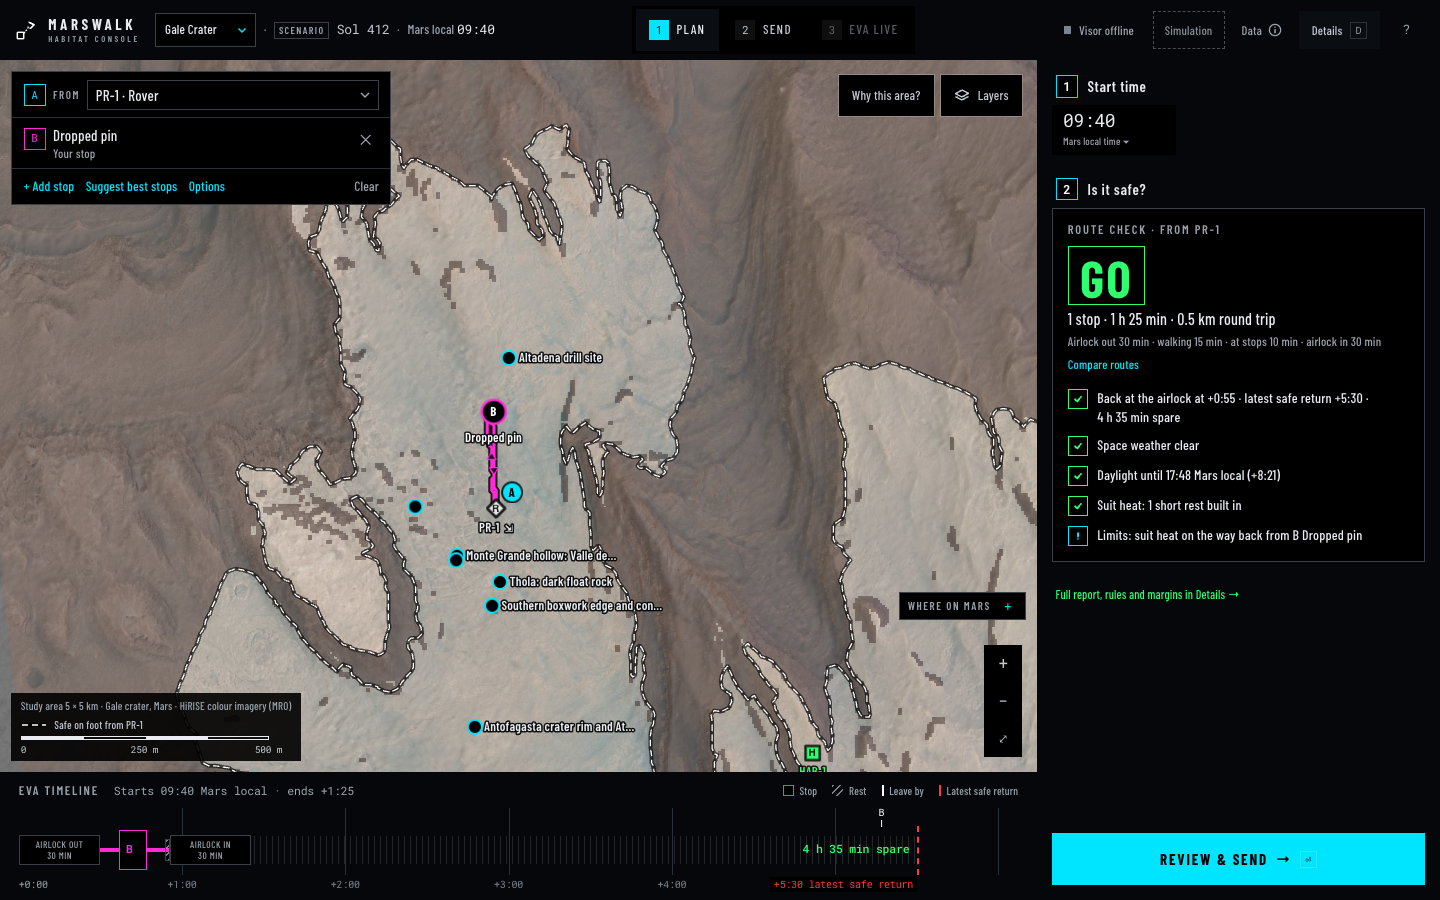
\includegraphics[width=\textwidth]{console-go.png}
    \caption{Plan mode: a \go verdict for a pin staged from PR-1.}
  \end{subfigure}\hfill
  \begin{subfigure}[b]{0.365\textwidth}\centering
    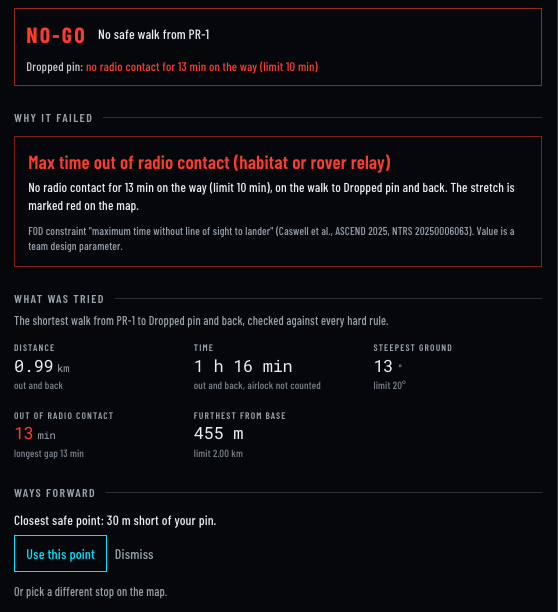
\includegraphics[width=\textwidth]{console-nogo-details.png}
    \caption{A \nogo explained.}
  \end{subfigure}
  \caption{Habitat console at Gale. (a) The IV picks a base and drops a pin. The verdict card lists the latest safe return, space weather, daylight and suit-heat rests. The dashed outline is the area walkable under the per-cell constraints, the magenta line is the route, and the timeline shows the airlock periods and the latest safe return. (b) For a pin in a radio shadow, the details drawer names the failing rule (13\,min without contact against a limit of 10) and its source, reports what was tried, and offers the closest safe point, which the engine has re-planned and confirmed.}
  \label{fig:console}
\end{figure*}

\paragraph{Habitat console.} The console asks one question at a time and moves through three modes: \emph{Plan}, \emph{Send} and \emph{EVA live} (\cref{fig:console}). Interaction follows familiar consumer map conventions. The IV sets a base and destinations, searches named places or drops a pin anywhere, and each pin gets an immediate safety preview. Science stations appear as suggested places, but any destination the IV picks is treated as must-visit: if it is infeasible, the console explains why instead of dropping it. The verdict comes first, in plain terms such as ``what limits this walk'', ``leave-by time'' and ``no safe walk from here''. A ``Why this area?'' sequence shrinks the walkable area one constraint at a time and cites the source of each limit. For a \nogo, the console marks the failing stretch of the route in red and offers two ways forward: the closest safe point and a better rover position. A rules view lists all twelve constraints with their evidence classes, and an evidence panel states what is measured and what is assumed. In the end-to-end test the verdict appears 2.1\,s after page load with no clicks, a plan reaches crew acceptance in three clicks, and an emergency re-route takes two.

\newcommand{\phoneshot}[2]{\tikz[baseline]{\node[inner sep=0pt] (img) {\includegraphics[height=#2]{#1}};
  \draw[ink, line width=2.2pt, rounded corners=7pt] ([shift={(-1.6pt,-1.6pt)}]img.south west) rectangle ([shift={(1.6pt,1.6pt)}]img.north east);}}
\begin{figure*}[t]
  \centering
  \begin{subfigure}[t]{0.24\textwidth}\centering
    \phoneshot{ar-nav.jpg}{70mm}
    \caption{Navigating.}
  \end{subfigure}\hfill
  \begin{subfigure}[t]{0.24\textwidth}\centering
    \phoneshot{ar-reroute.jpg}{70mm}
    \caption{Off route: local re-route.}
  \end{subfigure}\hfill
  \begin{subfigure}[t]{0.24\textwidth}\centering
    \phoneshot{ar-linklost.jpg}{70mm}
    \caption{Link lost: autonomous.}
  \end{subfigure}
  \caption{Phone AR navigator during a simulated walk on the Gale pack, served by the real habitat server; the camera feed is a Curiosity Mastcam frame (sol 5072) and the heading is simulated. (a) Chevrons on the ground bend toward the next steer point; one instruction card gives the target, and the top bar shows distance, arrival time, position uncertainty, elapsed time, heading and course. (b) After the walker is pushed 43\,m off the route, the phone re-plans locally with the engine's A$^\ast$ (``New route: 155\,m, about 5\,min'') and draws the new path. (c) With the link down, the navigator turns white and declares itself autonomous on the last confirmed route.}
  \label{fig:navigator}
\end{figure*}

\paragraph{Navigator.} The astronaut's navigator is a phone AR application (\cref{fig:navigator}). It uses the same flight logic as a full-screen visor display that we also built: link handling, the route state machine, the safety core, store-and-forward telemetry and crash-safe checkpoints. The rear camera fills the screen, and only glanceable cues are drawn over it. If the astronaut strays from the route, the phone re-plans locally with the engine's A$^\ast$ \citep{hart1968}, with the same cost and blocking, and the heat governor still inserts rests (\cref{sec:heat}). Three voice commands (``accept route'', ``task done'', ``depart'') replace taps that suited crew cannot make. When the link has been down for 3\,s, the navigator declares itself autonomous and keeps guiding on the last confirmed route with its safety core. The walker is simulated, and the AR navigator has no automated tests yet.

\begin{figure*}[t]
  \centering
  % Suit hardware concept (team concept study), redrawn: (a) helmet optics, (b) localization without GPS, (c) suit compute, radio and power.
% Solid cyan boxes run in the software today with simulated sensor inputs; dashed boxes are hardware concept.
\begin{tikzpicture}[x=1mm, y=1mm, font=\rmfamily\fontsize{6}{7}\selectfont,
  impl/.style={draw=accent, line width=0.6pt, fill=accent!8, rounded corners=1.5pt, align=center, inner sep=2.2pt,
               execute at begin node={\hyphenpenalty=10000\linespread{0.95}\selectfont}},
  conc/.style={draw=ink!55, dashed, line width=0.55pt, fill=white, rounded corners=1.5pt, align=center, inner sep=2.2pt,
               execute at begin node={\hyphenpenalty=10000\linespread{0.95}\selectfont}},
  arr/.style={-{Stealth[length=3.2pt]}, line width=0.5pt, draw=ink!65},
  lab/.style={font=\rmfamily\fontsize{6}{7}\selectfont, text=ink!75, fill=white, inner sep=0.8pt},
  ptitle/.style={font=\rmfamily\bfseries\scriptsize, text=ink, anchor=west},
  note/.style={font=\rmfamily\itshape\fontsize{6}{7}\selectfont, text=muted, anchor=west},
]
\newcommand{\bx}[2]{{\scriptsize\textbf{#1}}\\[0.6pt]#2}
% ===================== (a) helmet optics =====================
\node[ptitle] at (0,101) {(a) Monocular AR helmet optics};
\draw[ink!35, dashed, line width=0.5pt] (40,82) ellipse (41 and 15.5);
\node[note] at (24,96) {pressurized helmet envelope};
\node[conc, text width=21mm] (lcos) at (14,84) {\bx{LCoS light engine}{illumination, microdisplay, projection and collimation}};
\node[conc, text width=23mm] (wg) at (45,84) {\bx{Reflective waveguide}{coupling, internal reflection, partially reflective out-coupler}};
\draw[ink!70, fill=paper3, line width=0.5pt] (72,84) ellipse (4 and 3);
\fill[ink!85] (73,84) circle (1.6);
\node[font=\rmfamily\bfseries\fontsize{6}{7}\selectfont, text=ink] at (72,78.4) {eye};
\draw[arr] (lcos) -- node[lab, above=1pt] {pixels} (wg);
\draw[arr] (wg) -- node[lab, above=1pt] {virtual image} (67.6,84);
\draw[arr, ink!45] (86,88.5) -- node[lab, above=0.5pt, pos=0.35] {terrain view} (76.2,85.2);
\node[conc, text width=27mm] (dif) at (17,67) {\bx{Display interface}{wired video from the suit computer, helmet-safe routing}};
\node[conc, text width=29mm] (oc) at (56,67) {\bx{Optical constraints}{eye relief, eyebox, bright sunlight, field of regard, fogging}};
\draw[arr] (dif.north) -- (dif.north |- lcos.south);
\draw[arr] (oc.north) ++(8,0) -- (72,80.8);

% ===================== (c) suit compute, radio, power =====================
\node[ptitle] at (91,101) {(c) Suit compute, radio and power};
\node[conc, text width=17mm] (sens) at (101,88) {\bx{IMUs, cameras}{sensor streams}};
\node[conc, text width=30mm, minimum height=15mm] (soc) at (131,86.5) {\bx{Embedded CPU/GPU}{dead reckoning and fusion, periodic map matching, route tracking, HUD graphics, telemetry}};
\node[conc, text width=15mm] (hud) at (163,88) {\bx{HUD driver}{video to the waveguide}};
\node[conc, text width=17mm] (wd) at (101,74) {\bx{Watchdog}{reset, fault inhibit}};
\node[conc, text width=19mm] (pwr) at (102,59.5) {\bx{Suit power tap}{protection, DC/DC}};
\node[conc, text width=24mm] (mem) at (131,59.5) {\bx{RAM and flash}{route, map tiles, telemetry queue, logs}};
\node[conc, text width=20mm] (rad) at (159,59.5) {\bx{Radio}{antenna, link supervision}};
\draw[arr] (sens) -- (soc.west |- sens);
\draw[arr] (soc.east |- hud) -- (hud);
\draw[arr] (wd.east) -- ([yshift=-4mm]soc.west);
\draw[arr] (pwr.north) -- ([xshift=-10mm]soc.south);
\draw[arr, {Stealth[length=3.2pt]}-{Stealth[length=3.2pt]}] (mem.north) -- (soc.south);
\draw[arr, {Stealth[length=3.2pt]}-{Stealth[length=3.2pt]}] (rad.north) -- ([xshift=10mm]soc.south);
\draw[arr] ([xshift=-3mm]rad.north east) -- ++(0,6) node[lab, above=0pt] {to habitat};
\node[note] at (91,51) {navigation and HUD stay local; the habitat supervises but is not in the control loop};

% ===================== (b) localization =====================
\draw[rule, line width=0.4pt] (0,47.5) -- (177,47.5);
\node[ptitle] at (0,44) {(b) Localization without GPS or a magnetic compass};
\node[conc, text width=21mm] (imu) at (12,33) {\bx{Boot IMUs}{6-axis, one per boot}};
\node[conc, text width=29mm] (pdr) at (49,33) {\bx{Pedestrian dead reckoning}{steps, stride, heading; zero-velocity updates at foot contact}};
\node[conc, text width=21mm] (cam) at (12,15) {\bx{Stereo cameras}{terrain imagery}};
\node[conc, text width=29mm] (vo) at (49,15) {\bx{Visual processing}{visual odometry; periodic matching to preloaded orbital imagery}};
\node[impl, text width=28mm] (fix) at (78,4.5) {\bx{Fixes and heading}{station arrival, landmark or rover ranging; Sun azimuth}};
\node[impl, text width=29mm, minimum height=21mm] (est) at (107,24) {\bx{Position estimate}{today: simulated drift and scripted fixes, with uncertainty; with hardware: fuse sensors, reject inconsistent fixes}};
\node[impl, text width=33mm, minimum height=21mm] (out) at (158,24) {\bx{Navigator and safety core}{route cue and uncertainty on screen; walk-back and shelter margins; off route $>$25\,m for 3\,s $\rightarrow$ local A$^\ast$; telemetry to the habitat}};
\draw[arr] (imu) -- node[lab, above=1pt] {inertial} (pdr);
\draw[arr] (cam) -- node[lab, above=1pt] {imagery} (vo);
\draw[arr] (pdr.east) -- node[lab, above=1pt] {high rate} ([yshift=5mm]est.west);
\draw[arr] (vo.east) -- node[lab, below=1pt] {when trusted} ([yshift=-5mm]est.west);
\draw[arr] (fix.east) -| (est.south);
\draw[arr] (est) -- node[lab, above=1pt] {pose and covariance} (out);
% legend
\node[impl, minimum width=5mm, minimum height=2.6mm, inner sep=0pt] at (129,4.5) {};
\node[note] at (132.5,4.5) {runs in the software today (simulated inputs)};
\node[conc, minimum width=5mm, minimum height=2.6mm, inner sep=0pt] at (129,-0.5) {};
\node[note] at (132.5,-0.5) {hardware concept, not yet built};
\end{tikzpicture}

  \caption{Suit hardware concept and GPS-free localization, redrawn from the team's concept study \citep{marswalkconcept2026}. (a) Monocular AR helmet optics. (b) Localization: solid boxes run in the software today with simulated sensor inputs; dashed boxes are hardware concept. (c) Suit compute, radio and power. This is a proposed architecture: no processor, power budget or radio design has been selected or qualified.}
  \label{fig:hardware}
\end{figure*}

\subsection{Positioning without GPS, and suit hardware}
\label{sec:hardware}
Mars has no satellite navigation and no Earth-like global magnetic field. Yet the navigator must know where the astronaut is to look up walk-back and shelter margins, detect a wrong turn and report position to the habitat. \Marswalk therefore treats position as an estimate with an uncertainty, never as a fact (\cref{fig:hardware}b).

In the software today, the navigator keeps the simulated true position separate from its estimate. The estimate drifts by about 2\,m per minute walked, a team assumption in the range of foot-mounted inertial dead reckoning \citep{yamagishi2022pdr}. Every 10 minutes a landmark sighting or radio ranging to the rover corrects it, as does each arrival at a station, resetting the error to 1.5\,m; both kinds of fix are scripted in simulation. The display shows the current uncertainty and the time since the last fix (\cref{fig:navigator}). If the estimate leaves the route by more than 25\,m for 3\,s, the phone re-plans locally with A$^\ast$ to the next stop or to shelter. The visor display takes its heading reference from the Sun's azimuth, computed from solar longitude and local time, with landmark bearings near noon; the phone uses its compass, which works only on Earth, as a demo convenience.

The team's concept study sketches the suit hardware that would supply these measurements \citep{marswalkconcept2026}. A 6-axis inertial measurement unit (IMU) on each boot feeds pedestrian dead reckoning, with zero-velocity updates at each foot contact. Stereo helmet cameras give visual odometry and, periodically, an absolute fix by matching camera views to preloaded orbital imagery. In the concept, a state estimator fuses accepted measurements, rejects inconsistent ones and outputs position, heading and uncertainty. An embedded computer holds the route and orbital map tiles and runs fusion, route tracking and display graphics behind an independent watchdog. It talks to the habitat over a supervised radio link; the habitat supervises but is never in the high-rate loop, and during an outage it marks the last reported position as stale instead of implying live tracking. A monocular LCoS light engine and a reflective waveguide place a virtual cue over one eye. NASA's Joint AR pilot, which tested a different display on an Earth analog, motivates a display of this kind: with five astronaut-office crew on an Earth analog, median navigation time fell from 15.87 to 13.20 minutes compared with a paper map, and median distance from planned waypoints fell from 4.47 to 1.79\,m \citep{smith2026jointar}. The main risks are fitting the display into the helmet (eye relief and eyebox), aligning the heading cue, since a misaligned cue can be worse than none, and map matching on featureless or shadowed terrain. None of this hardware has been built or tested.

\section{Evaluation}
\label{sec:eval}

We ask five questions. Do the models agree with measured NASA data? Are search and selection correct? What does constraint-aware planning change? Does an independent implementation agree? Does the end-to-end system meet its budgets? \Cref{tab:evidence} summarizes the answers. We say a model \emph{reproduces} or is \emph{compared with} data; none of these checks validates the system for crewed use.

\begin{table*}[t]
  \centering\small
  \caption{Summary of the evidence. MAPE: mean absolute percentage error; MAE: mean absolute error; pp: percentage points. ``By construction'' means the property follows from the design and is checked by tests.}
  \label{tab:evidence}
  \begin{tabularx}{\textwidth}{@{}>{\raggedright\arraybackslash}p{0.26\textwidth} L L@{}}
    \toprule
    Check & Result & Main caveat \\
    \midrule
    Walking energy vs NASA suited data & MAPE 10.6\% at 0.22--0.32\,$g$ (17.6\% at our pace); 36.0\% at 0.12--0.17\,$g$ & Digitized trend lines; level walking under-predicted; 0.38\,$g$ extrapolated \\
    Terrain sky obstruction vs \citet{guo2026} & MAE 2.0\,pp, $r=0.94$ (15 periods) & Normalization chosen after seeing the data; one miss of 12\,pp \\
    Dose vs Curiosity RAD, year 1 & 198.8 vs 207.8\,µGy/day ($-4.3$\%) & $-8.7$\% at the scenario season; $-20$\% to $+41$\% over the solar cycle \\
    Leg search vs independent oracle & A$^\ast$ optimality gap 0.000\% (80 Gale cases) & One site, one seed \\
    Station selection vs brute force & Equal on 320 random instances & Up to seven stations \\
    Slope-masked routing & 75\% of routes contain a step over 20$^\circ$; 199 of 200 break a constraint & Naive baseline by design \\
    Science when time is short & $+5.0$\% (95\% CI 3.9--6.1\%) vs a checked greedy planner; never lower & Team science values \\
    Staging (Hab-1 vs PR-1) & Habitat infeasible under every single relaxation tested; rover feasible & One scenario habitat position \\
    Engine vs independent checker & Agree on 23 of 24 walks; the miss is a safe-side \nogo & 24 single-destination walks \\
    End-to-end system & Package 10,994\,B; visor link loss to autonomous 3.4\,s; re-plan 8.3\,ms median & One local run; no radio hardware \\
    \bottomrule
  \end{tabularx}
\end{table*}

\subsection{Physical models against measured data}
\label{sec:eval-models}

\begin{figure*}[t]
  \centering
  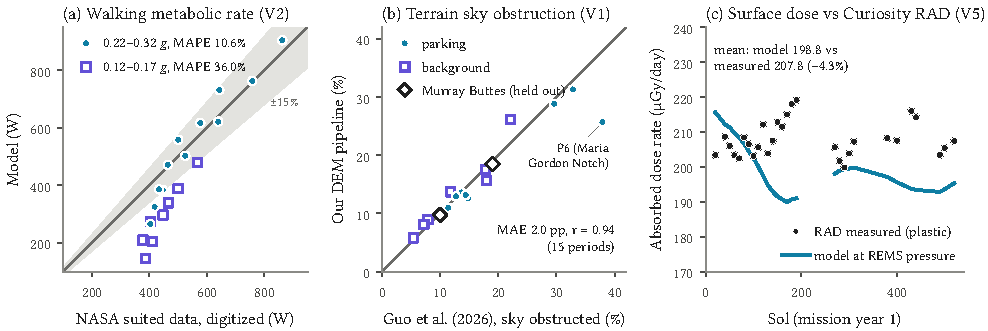
\includegraphics[width=0.92\textwidth]{eval_models.pdf}
  \caption{Model checks against measured NASA data. (a) Suited metabolic rate: model against NASA suited partial-gravity data \citep{norcross2010incline}, digitized from published trend lines (five gravity levels, four grades; band $\pm15$\%). (b) Terrain sky obstruction at Curiosity's parking positions and background periods against \citet{guo2026}; Murray Buttes was held out (reference value from \citealt{ehresmann2021}). (c) Daily absorbed dose in the RAD plastic detector over Curiosity's first Mars year against our model at measured REMS pressure.}
  \label{fig:models}
\end{figure*}

\paragraph{Walking energy.} NASA's Integrated Suit Test~2 measured six astronauts walking in a 121\,kg suit at 0.12--0.32\,$g$ on grades of 0--30\% \citep{norcross2010incline}. No table of means exists, so we digitized the per-gravity trend lines (point error about $\pm4$\% of power). We ran the model without fitting, using the subjects' mean mass of 80.7\,kg, no tools, $\eta=1$ and 0.765\,m/s, the midpoint of the reported speeds. At 0.22--0.32\,$g$ the MAPE is 10.6\%; at 0.56 and 0.97\,m/s, the ends of the speed range, it is 17.6\% and 18.7\%. At 0.12--0.17\,$g$ it is 36.0\% (\cref{fig:models}a). The model under-predicts level walking (by 34\% at 0.22\,$g$ and 62\% at 0.12\,$g$). The measured data show a floor of oxygen uptake that barely changes with gravity, whereas scaling the whole equation by $g$ drives the standing terms toward zero.

\paragraph{Terrain shielding.} \Citet{guo2026} tabulate the sky obstructed by terrain at Curiosity's parking positions and the resulting dose drops. Our pipeline casts rays from 1\,m above the DEM at Curiosity's waypoints. It reproduces the 15 obstruction values with an MAE of 2.0\,pp and $r=0.94$ (\cref{fig:models}b). We chose a solid-angle normalization after seeing the comparison; the two alternatives give 6.5 and 11.9\,pp. The largest miss, 12\,pp, is the narrow Maria Gordon notch. For held-out Murray Buttes we obtain 18.5\% obstruction against 19\% reported, but predict a dose drop of 8.4\% against a measured 4\%. Predicted drops have an RMSE of 4.3\,pp, against 5.1\,pp for always predicting the mean, so the shielding layer is labelled indicative.

\paragraph{Surface dose.} We compared the dose model with RAD daily dose \citep{hassler2012} on 29 first-year sols that have REMS pressure, excluding sols that a simple heuristic flags as affected by solar particle events. The measured mean is 207.8\,µGy/day and the model gives 198.8\,µGy/day ($-4.3$\%; \cref{fig:models}c). The first-year data imply $\Phi\approx518$\,MV rather than the assumed 600\,MV, which explains most of the bias. At the scenario season the model is 8.7\% low. Later years at the same season range from $-20$\% to $+41$\% of the first-year value, so route doses are indicative to a few tens of percent.

\subsection{Correctness of search and selection}
\label{sec:eval-planner}
A benchmark runs each search and cost model over 40 static and 40 hidden-hazard scenarios on the Gale grid. It scores paths against an independently written Dijkstra oracle (\cref{tab:bench} in \cref{app:tables}). A$^\ast$ is exactly optimal and expands about a quarter as many nodes as the engine's Dijkstra, whose 0.036\% gap we attribute to decisecond quantization. A slope-weighted cost model typical of generic tools finds paths that look 5\% cheaper only by taking 140--166 steps over the 20$^\circ$ step limit. The station DP equals brute force on 320 instances, and the property test in \cref{sec:sim} found no unsafe plan. All 138 unit tests passed on 15 November 2026.

\subsection{What constraint-aware planning changes}
\label{sec:eval-impact}

\begin{figure*}[t]
  \centering
  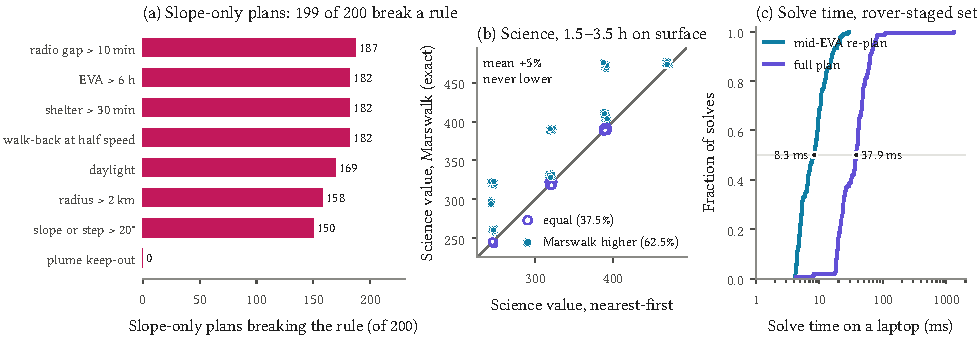
\includegraphics[width=0.92\textwidth]{eval_impact.pdf}
  \caption{Planning impact over simulated EVAs at Gale. (a) Slope-masked least-cost plans (200 rover-staged scenarios) that break each constraint when replayed in our simulator. (b) Science value of exact selection against a nearest-first planner with the same checks, with 1.5--3.5\,h of surface time (200 scenarios, jittered). (c) Solve times on a laptop.}
  \label{fig:impact}
\end{figure*}

We generated scenarios on the Gale pack with fixed seeds. The main set has 200 rover-staged EVAs requesting 3--6 of the 12 stations (60 more from the habitat). An oversubscribed set offers all 12 stations but leaves only 90--210\,min (1.5--3.5\,h) of surface time. \emph{Slope-masked} routing visits all requested stops along least-cost paths on a grid that blocks slopes over 20$^\circ$; it is naive by design. \emph{Nearest-first} adds the nearest stop only if the whole plan passes our checker; it is a greedy baseline with a perfect rule checker, which no human planner has.

Replayed in our simulator, 199 of 200 slope-masked plans break at least one constraint (\cref{fig:impact}a), mostly constraints that slope cannot see: radio gap (187), walk-back, shelter and EVA duration (182 each). Of the 200 routes, 150 (75\%) contain a step steeper than 20$^\circ$ between two cells that each pass the cell-slope mask. \Marswalk and nearest-first return no violating plan by construction; \cref{sec:eval-crosscheck} tests the checker independently. With a full EVA, the constraints are tight enough that nearest-first picks the same stations as \Marswalk in all 200 scenarios. When time is short, exact selection gains 5.0\% science value on average (paired bootstrap 95\% CI 3.9--6.1\%, median 1.1\%, maximum 30.6\%). It is better in 62.5\% of scenarios and never worse (\cref{fig:impact}b). Full plans take a median of 37.9\,ms and mid-EVA re-plans 8.3\,ms on a laptop (\cref{fig:impact}c), fast enough to re-plan on every telemetry update.

\subsection{Staging: habitat or rover}
\label{sec:eval-scenario}

\begin{figure*}[t]
  \centering
  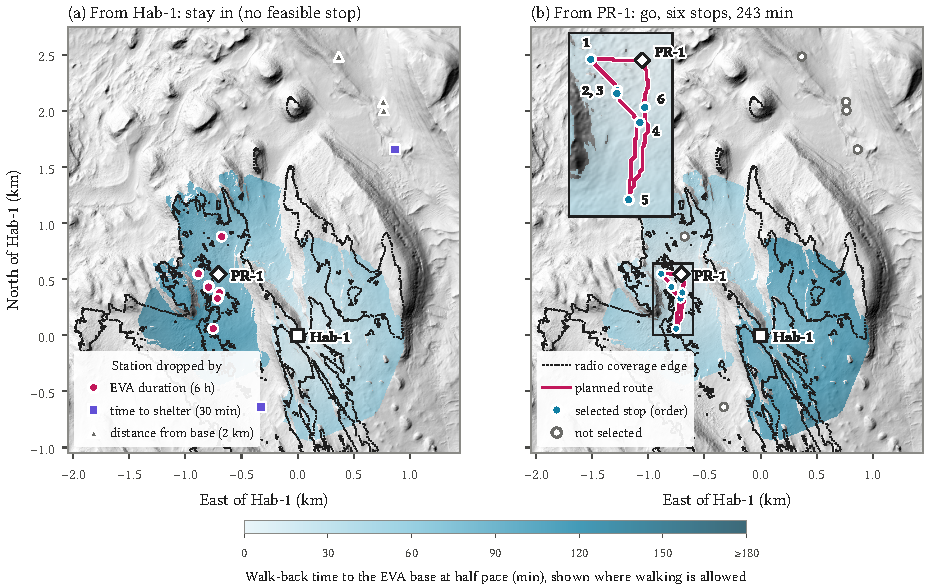
\includegraphics[width=0.78\textwidth]{scenario.pdf}
  \caption{The default scenario, planned by the engine. Shading: walk-back time to the EVA base where walking is allowed; dotted lines: edge of radio coverage. (a) From Hab-1 every station fails: seven exceed the 6-hour EVA once heat rests on the climb back are included, two exceed 30\,min to shelter and three lie beyond 2\,km. (b) From PR-1, a six-stop plan in 243\,min (inset: route and order; stops 2 and 3 are about 10\,m apart). The walkable footprint is the same from both bases. What differs is the time to get back: 80--115\,min from stations ST01--ST07 to Hab-1, against 8--30\,min to PR-1.}
  \label{fig:scenario}
\end{figure*}

The default scenario plans all twelve stations from the habitat at 09:40 LTST (\cref{fig:scenario}). The engine returns \stayin with EVA duration as the binding constraint, and adds that staging from the rover allows six stations. The seven boxwork stations lie 144--217\,m below the habitat and 0.75--1.1\,km away, so every walk to them ends in a loaded climb at 668--824\,W, roughly twice the heat budget. Staged from PR-1, the plan visits ST04, ST02, ST03, ST06, ST07 and ST05 for a science value of 475 in a 243-minute EVA (183\,min on the surface, including 9.5\,min of heat rests; \cref{fig:anatomy}). It never goes more than 487\,m from the rover, and its binding constraint is the radio gap, with a margin of 0.4\,min.

\begin{figure*}[t]
  \centering
  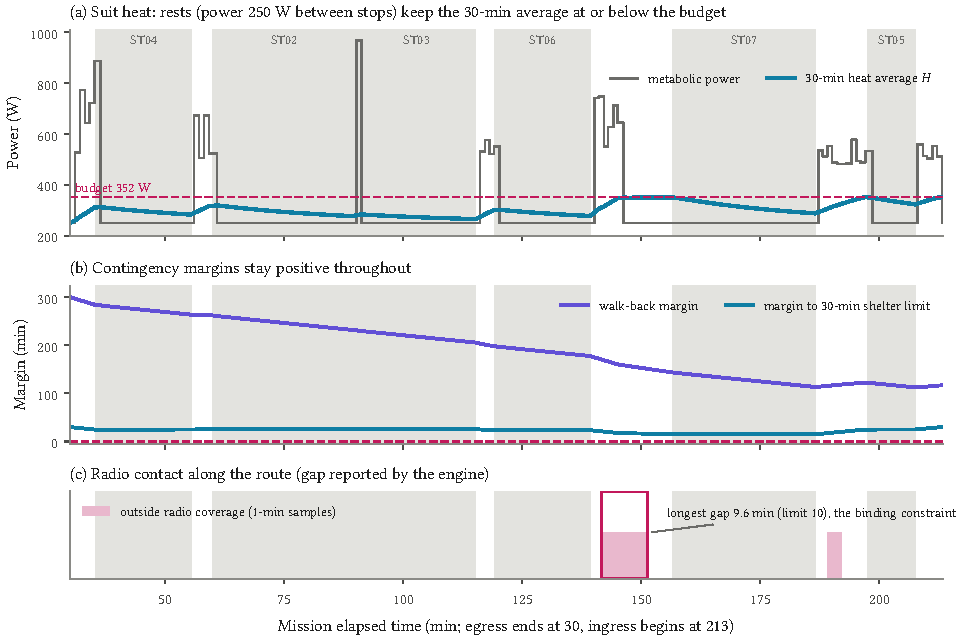
\includegraphics[width=0.72\textwidth]{anatomy.pdf}
  \caption{Anatomy of the six-stop plan from PR-1, from the engine's burndown (grey bands: stations). (a) Metabolic power and its 30-minute average against the 352\,W budget; rests at 250\,W between stops total 9.5\,min. (b) Walk-back margin and margin to the shelter limit. (c) Samples outside radio coverage; the engine's longest gap, 9.6\,min against a limit of 10, is the binding constraint.}
  \label{fig:anatomy}
\end{figure*}

\Cref{tab:sensitivity} varies one team-chosen parameter at a time. From the habitat, no single change makes any station walkable. Raising the heat budget to 530\,W, or removing it, turns the seven boxwork failures into radio-gap failures. Relaxing the radio gap alone leaves them failing on EVA duration. The walk-back pace, shelter limit and radius only change which of the other five stations fails first. Only lifting both the heat and radio-gap limits makes six stations walkable from the habitat. The boxwork stations are therefore blocked jointly by suit heat and radio contact, which a single-rule binding constraint cannot express. From the rover, the plan is robust to these parameters, and relaxing either heat or radio gap adds ST01 (value 555). Per-cell rules alone do not separate the two bases. From either base, the same 2.86\,km$^2$ and seven stations satisfy slope, keep-out, radius, shelter and out-and-back time (\cref{tab:ablation}). The difference arises only from constraints evaluated along the trajectory, which is why the simulator matters. This is our model's result for one habitat position, not a NASA finding. It agrees with DRA~5.0's use of pressurized rovers as mobile bases \citep{drake2009dra5} and shows that a crew-side planner can answer where to stage a walk, not only how to walk it.

\begin{table*}[t]
  \centering\small
  \caption{One-at-a-time sensitivity of the default scenario (all twelve stations, 09:40 LTST). Dropped: stations dropped per rule (EVA = duration, radio = radio gap, w-b = walk-back).}
  \label{tab:sensitivity}
  \begin{tabular}{@{}l l c c c l@{}}
    \toprule
    Base & Variant & Result & Stops & Value & Dropped \\
    \midrule
    Hab-1 & baseline & \stayin & 0 & -- & 7 EVA, 2 shelter, 3 radius \\
          & heat budget 530\,W, or heat limit off & \stayin & 0 & -- & 7 radio, 2 shelter, 3 radius \\
          & radio gap 20\,min, or radio-gap rule off & \stayin & 0 & -- & 7 EVA, 2 shelter, 3 radius \\
          & walk-back pace $0.67\times$ & \stayin & 0 & -- & 7 EVA, 2 shelter, 3 radius \\
          & shelter limit 45\,min & \stayin & 0 & -- & 7 EVA, 1 radio, 1 shelter, 3 radius \\
          & radius 3\,km & \stayin & 0 & -- & 7 EVA, 5 shelter \\
          & heat limit and radio-gap rule both off & \go & 6 & 470 & 1 w-b, 2 shelter, 3 radius \\
    \midrule
    PR-1  & baseline & \go & 6 & 475 & 1 radio, 2 shelter, 3 radius \\
          & heat budget 530\,W, or heat limit off & \go & 7 & 555 & 2 shelter, 3 radius \\
          & radio gap 20\,min, or radio-gap rule off & \go & 7 & 555 & 2 shelter, 3 radius \\
          & walk-back pace, shelter limit or radius (as above) & \go & 6 & 475 & radius and shelter drops shift \\
    \bottomrule
  \end{tabular}
\end{table*}

\subsection{Independent cross-check}
\label{sec:eval-crosscheck}
We sampled 24 single-destination walks at Gale: 12 \go and 12 \nogo, with the \nogo cases spread across the failing rules. An independently written Python checker decodes the site pack itself and recomputes slope, step grades, line of sight (with curvature), keep-outs, sun elevation, walk-back and shelter times. It shares only route cells, rule values, mast positions and rasters with the engine, and it omits the heat governor. Engine and checker agree on 23 of 24 walks, and on all 96 rule-level checks that do not depend on heat rests (no walk fails slope or keep-out, so only radius and shelter discriminate). In the one disagreement, the engine called a walk \nogo because its heat-aware route spent 0.22\,min too long out of contact. The shortest-time path stays within the limit, and the engine's own simulator confirms it passes, but the planner did not try it. The error is on the safe side. Two blind AI judges, given the rules and engine-generated evidence, matched the same 23 verdicts. They test rule application only, and they share a model family with the agents that wrote much of the code.

\subsection{End-to-end system}
\label{sec:eval-system}
An automated test runs the habitat server, console and visor as three local processes with the real engine and the Gale pack (one run). The phone navigator reuses the visor's controller but is not part of this test, so these figures are for the visor. The first plan solves cold in 1.6\,s. The signed 10,994-byte package is verified on the visor 168\,ms after ``Send to crew''. A simulated radiation spike produces a return route in 2\,ms (668\,ms to the screen). After a link drop the visor becomes autonomous in 3.4\,s, and queued telemetry back-fills within 1.8\,s of recovery. These timings come from a local network, not from radio hardware.

\section{Discussion}
\label{sec:discussion}

\paragraph{What the results show.} At a real Mars site, the constraints, not the optimizer, decide most plans. A naive slope-masked planner broke documented constraints almost every time, mostly ones slope never sees, and three quarters of its routes contained steps that cell-slope masks miss. A greedy planner with the same checks matched exact selection whenever time was plentiful. The value of a crew-side planner therefore lies first in checking constraints and explaining them, and second in optimizing science, where exact selection helped when time was short. The staging result shows why checks must run along the trajectory: per-cell rules make the habitat and the rover look identical, while heat rests and accumulated radio gaps separate them. Suit thermal capacity and communications coverage also interact. From the habitat, raising the heat budget only exposed the radio limit, while from the rover a 530\,W budget added a seventh stop.

\paragraph{Why the architecture fits Mars.} Earth cannot answer in time, the helmet cannot afford dense fields, and the link will drop behind terrain. A signed package with a conservative coarse grid lets the navigator make the decisions that cannot wait, such as whether the crewmember is still within walk-back and shelter limits and which way is home, with no link and no habitat computation. The same split would serve lunar operations where line of sight to the base is intermittent.

\paragraph{Limitations.} No suited person has walked a \Marswalk plan, no EVA operator has used the console, and the explanations are untested with users. The walker in our tests is a simulator that uses the engine's own power model. The simulator shares models with the planner, so it catches search errors, not model errors. The metabolic model extrapolates to Mars gravity and under-predicts level walking. Its standing cost (474\,W) exceeds both the heat budget and the 250\,W rest power we assume, and the 30-minute window, rest power and initial heat state were not varied. Walk-back and shelter fields ignore heat rests, which presumes that contingency returns may exceed the nominal heat budget. Oxygen is a time budget, not a consumables model. Line of sight ignores curvature, Fresnel clearance and link budget, and the rover relay is assumed. Three constraint values are team parameters, and the station values are a team heuristic. Station selection is exact only over precomputed legs and up to 15 candidates, and exactness was tested against brute force only up to seven stations. The link is a local WebSocket, not a radio. Only route integrity is protected; the link is unencrypted and consoles are unauthenticated. The AR navigator's positioning is simulated, and the suit hardware is a concept. The impact and sensitivity studies use one site, one habitat position and single end-to-end runs.

\paragraph{Next steps.} The most valuable next steps are human-in-the-loop: replaying analog EVA data through the engine and putting the console in front of EVA operators. On the modelling side, the obvious checks are a gravity-independent floor for walking energy and comparisons with NASA's own regression for the suited data and with Apollo EVA metabolic rates \citep{waligora1975}. Further steps are heat-aware contingency fields, radio-aware routing and a sweep over habitat positions. On the hardware side, the concept study proposes replaying recorded boot-IMU and camera data through the estimator, an analog walk with surveyed checkpoints, worst-case reconnection tests and helmet readability trials. The pipeline accepts any digital elevation model, so lunar sites are a natural second domain.

\section{Conclusion}
\label{sec:conclusion}
Mars crews will plan and carry out many of their own EVAs, with Earth up to 22 light-minutes away and out of reach near conjunction. \Marswalk shows that a crew-side planner for that job can be built from public NASA data, published physiology and well-understood algorithms. It plans against twelve sourced constraints, re-checks every plan in a separate simulator, explains each verdict, and hands the astronaut a signed route that keeps guiding without a link or GPS. Its models are compared with measured NASA data, and their errors are reported in \cref{sec:eval-models}. At Gale it yields a concrete staging result: relaxing either the heat limit or the radio-gap limit alone leaves the habitat walk infeasible, while a nearby pressurized rover makes a six-stop walk feasible. Suited people, real radios and EVA operators come next; the architecture, code and evidence are open for others to test and improve.


\appendix
\section{Candidate science stations}
\label{app:stations}
\Cref{tab:stations} lists the twelve candidate stations, their values and dwell times, their positions relative to both bases, and the engine's result for each in the default scenario.

\begin{table*}[t]
  \centering\footnotesize
  \caption{The twelve candidate stations in the \code{gale-v1} site pack, each a Curiosity target positioned from the rover's waypoint on the sol it was studied. Value (0--100) is the team's science-traceability heuristic, not a NASA ranking. $\Delta z$ and distances are relative to Hab-1 (and PR-1). The last two columns give the engine's result in the default scenario.}
  \label{tab:stations}
  \begin{tabularx}{\textwidth}{@{}l L r r r r r l l@{}}
    \toprule
    ID & Curiosity target & Value & Dwell (min) & $\Delta z$ (m) & Hab-1 (km) & PR-1 (km) & From Hab-1 & From PR-1 \\
    \midrule
ST01 & Altadena drill site (boxwork bedrock) & 80 & 25 & -217 & 1.11 & 0.34 & EVA duration & radio gap \\
ST02 & Monte Grande hollow: Valle de la Luna drill site & 95 & 30 & -184 & 0.91 & 0.14 & EVA duration & stop 2 \\
ST03 & Nevado Sajama ridge-top drill site & 90 & 25 & -181 & 0.90 & 0.15 & EVA duration & stop 3 \\
ST04 & Peace-sign ridge intersection and Laguna Miniques\ldots & 70 & 20 & -187 & 1.04 & 0.18 & EVA duration & stop 1 \\
ST05 & Thola: dark float rock (possible meteorite) & 60 & 10 & -182 & 0.79 & 0.16 & EVA duration & stop 6 \\
ST06 & Southern boxwork edge and contact with the\ldots & 75 & 20 & -177 & 0.79 & 0.22 & EVA duration & stop 4 \\
ST07 & Antofagasta crater rim and Atacama sulfate block & 85 & 30 & -144 & 0.75 & 0.49 & EVA duration & stop 5 \\
ST08 & Valle Grande: post-boxwork layered sulfate buttes\ldots & 65 & 20 & -45 & 0.72 & 1.24 & shelter time & shelter time \\
ST09 & Kings Canyon drill site (sulfate unit) & 60 & 20 & -247 & 1.87 & 1.92 & shelter time & shelter time \\
ST10 & Fascination Turret (upper Gediz Vallis ridge) & 70 & 25 & -296 & 2.15 & 2.07 & distance & distance \\
ST11 & Mineral King drill site (typical sulfate unit) & 72 & 20 & -302 & 2.22 & 2.13 & distance & distance \\
ST12 & Upper Gediz Vallis ridge float rocks (steep\ldots & 92 & 30 & -345 & 2.51 & 2.22 & distance & distance \\
    \bottomrule
  \end{tabularx}
\end{table*}

\section{Supporting tables}
\label{app:tables}
\Cref{tab:layers} lists every site-pack layer and its role, \cref{tab:bench} gives the leg-search benchmark, and \cref{tab:ablation} gives the per-cell constraint ablation discussed in \cref{sec:eval-scenario}.

\begin{table*}[t]
  \centering\footnotesize
  \caption{Layers in the Gale site pack and the decision each one changes. ``Indicative'' layers are labelled as such in the console. All products are public domain; the manifest records product identifiers, resolution, accuracy notes and SHA-256 digests. MRO: Mars Reconnaissance Orbiter; MEX: Mars Express; MGS: Mars Global Surveyor; MSL: Mars Science Laboratory; HiRISE: High Resolution Imaging Science Experiment; CTX: Context Camera; HRSC: High Resolution Stereo Camera; MOLA: Mars Orbiter Laser Altimeter; THEMIS: Thermal Emission Imaging System; CRISM: Compact Reconnaissance Imaging Spectrometer for Mars; REMS: Rover Environmental Monitoring Station.}
  \label{tab:layers}
  \begin{tabularx}{\textwidth}{@{}>{\raggedright\arraybackslash}p{0.2\textwidth} >{\raggedright\arraybackslash}p{0.27\textwidth} c L@{}}
    \toprule
    Layer & Mission / instrument & Native res. & Role in \Marswalk \\
    \midrule
    Elevation, slope, normals & MRO HiRISE + CTX, MEX HRSC, MGS MOLA (USGS merged DEM) & 1\,m & Walkable cells, step grade, 3-D step length, walking energy, radio viewshed, sun relief, pressure for dose \\
    Colour orthoimage & MRO HiRISE (78-quad colour basemap) & 0.25\,m & Base map, station context \\
    Thermal inertia & Mars Odyssey THEMIS & 100\,m & Terrain factor in walking cost (indicative) \\
    Sulfate, hydration signals & MRO CRISM (FRT000058A3) & 18\,m & Science context at each stop (indicative) \\
    Sky-view fraction & derived from the DEM & 5\,m & Terrain shielding of dose (indicative) \\
    Traverse, waypoints & MSL Curiosity (MMGIS) & ${\sim}$1\,m & Station positions, DEM check \\
    Point-of-view images & MSL Mastcam, Navcam & native & ``What you'll see'' at each stop \\
    Weather & MSL REMS (30 sols) & per sol & Conditions panel, season for sun geometry \\
    Space weather & CCMC DONKI (31 WSA--ENLIL runs, 2 flares) & event & Forecast \go/\textsc{caution} banner \\
    Sun position & Mars24 (NASA GISS) & --- & Daylight rule, lighting, heading cue \\
    Locator & Viking MDIM 2.1 & 232\,m & ``Where on Mars'' context \\
    \bottomrule
  \end{tabularx}
\end{table*}

\begin{table*}[t]
  \centering\footnotesize
  \caption{Leg-search benchmark on the Gale grid: 40 static and 40 hidden-hazard scenarios, scored under the Pandolf--Santee cost against an independent Dijkstra oracle. Latency is the median (p50) single-machine wall-clock time for static scenarios; hazard success is the share of hidden-hazard scenarios in which the walker reaches the goal. Violations are steps into blocked cells or over the 20$^\circ$ step grade, summed over all 80 scenarios.}
  \label{tab:bench}
  \begin{tabular}{@{}l l S[table-format=1.3] S[table-format=6.0] S[table-format=2.1] c S[table-format=3.0]@{}}
    \toprule
    Search & Cost model & {Gap (\%)} & {Expanded} & {p50 (ms)} & {Hazard success} & {Violations} \\
    \midrule
    A$^\ast$ & Pandolf--Santee & 0.000 & 73575 & 11.2 & 100\% & 0 \\
    Dijkstra (Dial) & Pandolf--Santee & 0.036 & 267523 & 36.0 & 100\% & 0 \\
    Weighted A$^\ast$ ($w=1.5$) & Pandolf--Santee & 2.847 & 44839 & 8.8 & 100\% & 0 \\
    A$^\ast$ & slope-weighted & {---} & 103593 & 31.0 & 100\% & 148 \\
    Dijkstra (Dial) & slope-weighted & {---} & 268407 & 79.4 & 100\% & 140 \\
    Weighted A$^\ast$ ($w=1.5$) & slope-weighted & {---} & 51228 & 14.9 & 100\% & 166 \\
    \bottomrule
  \end{tabular}
\end{table*}

\begin{table}[t]
  \centering\footnotesize
  \caption{Constraint ablation with per-cell rules only, applied in sequence: walkable area (km$^2$) and number of the twelve stations inside it, from each base. Trajectory constraints (heat rests, accumulated radio gap, daylight, EVA duration) are not included; they are what separate the two bases.}
  \label{tab:ablation}
  \begin{tabular}{@{}l S[table-format=2.2] c S[table-format=2.2] c@{}}
    \toprule
    & \multicolumn{2}{c}{From Hab-1} & \multicolumn{2}{c}{From PR-1} \\
    \cmidrule(lr){2-3}\cmidrule(lr){4-5}
    Rule added & {Area} & Stations & {Area} & Stations \\
    \midrule
    Walkable (slope, keep-out, data) & 17.71 & 12 & 17.71 & 12 \\
    + within 2\,km of the base & 9.75 & 9 & 9.39 & 9 \\
    + within 30\,min of a shelter & 2.86 & 7 & 2.86 & 7 \\
    + out-and-back in surface time & 2.86 & 7 & 2.86 & 7 \\
    + inside radio coverage & 1.56 & 7 & 1.56 & 7 \\
    \bottomrule
  \end{tabular}
\end{table}



\section*{Use of AI}
\addcontentsline{toc}{section}{Use of AI}
The problem, concept, system architecture and scope are the team's. Most of the software was written with Claude Code (Anthropic) coding agents under the team's direction and review, and AI assistance was used in drafting this paper; the team is responsible for its content. No AI model takes part in any safety decision in \Marswalk: routes are produced by the deterministic engine described in \cref{sec:engine}. AI-written code was reviewed by the team and is exercised by the unit, property and end-to-end tests and the independent checker reported here. Blind AI judges were used only as one of three checks of the engine's verdicts (\cref{sec:eval-crosscheck}); they belong to the same model family as the coding agents, which limits their independence. No AI-generated imagery appears in the system or in this paper; all images are NASA data or screenshots of the software.

\section*{Data and code availability}
The source code, site-pack manifests with product identifiers and SHA-256 digests, the check scripts and their results (in the \code{Validation/} directory), and the benchmark harness are available at \PaperRepo{} under the Apache-2.0 license. Site-pack rasters (about 58\,MB for Gale) are rebuilt from public sources by the included pipeline. Commands: \code{pnpm demo} (full system), \code{pnpm ci} (type check and unit tests), \code{pnpm e2e} (end-to-end test), \code{pnpm bench} (planner benchmark); the model and impact checks V1--V5 are under \code{Validation/}.

\section*{Data credits}
HiRISE: NASA/JPL-Caltech/University of Arizona. CTX, Mastcam: NASA/JPL-Caltech/MSSS. Navcam, Curiosity and Perseverance traverses: NASA/JPL-Caltech. HRSC: ESA/DLR/FU Berlin. THEMIS: NASA/JPL-Caltech/Arizona State University. CRISM: NASA/JPL-Caltech/JHU-APL. MOLA: NASA/GSFC. Gale merged DEM and Mars 2020 TRN products: USGS Astrogeology Science Center. RAD and REMS data: NASA Planetary Data System. Space-weather forecasts: NASA Community Coordinated Modeling Center (DONKI). Mars24: NASA Goddard Institute for Space Studies. This work is not endorsed by NASA.

\section*{Competing interests and funding}
The authors declare no competing interests. This work received no funding.

\section*{Acknowledgments}
We thank the organizers and mentors of the NASA International Space Apps Challenge Toronto local event, and the instrument and operations teams whose public data made this work possible.

\bibliographystyle{unsrtnat}
\bibliography{refs}

\end{document}
